\documentclass[t]{beamer}

\usetheme{Air}
\usepackage{graphics}
\usepackage{graphicx}
\graphicspath{{C:/Users/Brayden/Projects/PEPS-Data/}{.}}
%\usepackage{caption}
\usepackage{amsthm}
%\usepackage{thumbpdf}
\usepackage{wasysym}
\usepackage{ucs}
\usepackage[utf8]{inputenc}
\usepackage{pgf}
\usepackage{verbatim}
\usepackage{tikz}
\usepackage{pgfmath}
\usetikzlibrary{calc}
\usetikzlibrary{backgrounds}
\usetikzlibrary{arrows}
\usetikzlibrary{shapes.arrows}
\usetikzlibrary{shapes.geometric}
\usetikzlibrary{decorations.markings}
\usetikzlibrary{positioning}
\usetikzlibrary{fit,chains}
\usepackage{natbib}
\usepackage{wasysym}
\usepackage{soul} 
\bibliographystyle{apalike}  

%\usepackage{pstricks}
%\newpsobject{psid}{psline}{linestyle=dotted,dotsep=1pt}
%\newpsobject{pspsi}{psline}{doubleline=true}
%\newpsobject{pssigma}{psline}{linewidth=1.5pt}

%\usepackage{pgfpages}
%\setbeamertemplate{note page}[plain]
%\setbeameroption{show notes on second screen=right}
%http://tex.stackexchange.com/questions/21777/is-there-a-nice-solution-to-get-a-presenter-mode-for-latex-presentations

\newcommand{\beq}{\begin{equation}}
\newcommand{\eeq}{\end{equation}}
\newcommand{\beqa}{\begin{eqnarray}}
\newcommand{\eeqa}{\end{eqnarray}}
\newcommand{\bi}{\begin{itemize}}
\newcommand{\ei}{\end{itemize}}
\newcommand{\ket} [1] {\vert #1 \rangle}
\newcommand{\bra} [1] {\langle #1 \vert}
\newcommand{\braket}[2]{\langle #1 | #2 \rangle}
\newcommand{\ev}[1]{\langle #1 \rangle}
\newcommand{\vbra}[1]{\left ( #1 \right |}
\newcommand{\vket}[1]{\left |#1 \right )}
\newcommand{\vbraket}[2]{\left ( #1 \middle |#2 \right )} 
\newcommand{\braopket}[3]{\left \langle #1 \middle |#2 \middle | #3 \right \rangle} 
\newcommand{\vbraopket}[3]{\left ( #1 \middle |#2 \middle | #3 \right )} 

%\newcommand<>{\highlighton}[1]{%
%  \alt#2{\structure{#1}}{{#1}}
%}

\newcommand{\icon}[1]{\pgfimage[height=1em]{#1}}

\tikzset{peps/.style={circle=2pt,draw=black!100,fill=green!50,inner sep=3pt}}
\tikzset{bpeps/.style={circle=2pt,draw=black!100,thick,fill=green!50,inner sep=3pt}}
\tikzset{gamma/.style={circle=2pt,draw=black!100,fill=blue!20,inner sep=3pt}}
\tikzset{lambda/.style={rectangle,rotate=45,draw=black!100,fill=orange!50,inner sep=4pt}}
\tikzset{operator/.style={circle=2pt,draw=black!100,fill=orange!80,inner sep=3pt}}
\tikzset{cdot/.style={circle=2pt,draw=black!100,fill=white,inner sep=1pt}}
\tikzset{bg/.style={rounded corners,thin,fill=blue!10}}
\tikzset{inv/.style={opacity=0}}
\tikzset{spin/.style={circle=2pt,draw=black!100,fill=orange!80,inner sep=3pt}}
\tikzset{unitbox/.style={fill=black!3,rounded corners}}
\tikzset{corner/.style={rectangle=10pt,fill=blue!50,draw=black}}
\tikzset{side/.style={rectangle=6pt,fill=blue!20,draw=black}}
\tikzset{cside/.style={circle=6pt,fill=blue!20,draw=black}}
\tikzset{swapg/.style={circle=1pt,draw=black,fill=black!80,inner sep=1pt}}

\tikzset{base/.style={circle=2pt,fill=orange!80,draw=black}}
\tikzset{det/.style={circle=2pt,fill=blue!20,draw=black,inner sep=4pt}}
\tikzset{iso/.style={circle=2pt,fill=red!20,draw=black,inner sep=4pt}}
\tikzset{top/.style={circle=2pt,fill=black!20,draw=black,inner sep=4pt}}
\tikzset{siso/.style={circle=1pt,fill=red!20,draw=black,inner sep=1pt}}

%Brayden's
\tikzset{GHZ/.style={circle=2pt,fill=black!80,draw=black,inner sep=2pt}}
\tikzset{X/.style={circle=2pt,fill=black!80,text=white,font=\footnotesize, draw=black,inner sep=1pt}}
\tikzset{W/.style={circle=2pt,fill=black!20,draw=black,double,inner sep=2pt}}
\tikzset{eli/.style={ellipse, rotate=0, draw=black, fill=gray!20}}

%http://tex.stackexchange.com/questions/199683/how-to-plot-quantum-logical-gates-with-tikz
\tikzset{
cross/.style={path picture={ 
            \draw[thick,black](path picture bounding box.north) -- (path picture bounding                  box.south) (path picture bounding box.west) -- (path picture bounding                      box.east);
            }},
crossx/.style={path picture={ 
            \draw[thick,black,inner sep=0pt]
                (path picture bounding box.south east) -- (path picture bounding box.north west) (path picture bounding box.south west) -- (path picture bounding box.north east);
            }},
circlewc/.style={circle=2pt,draw, crossx}
}
%\newtheorem{LSM}{{\em Theorem: Lieb, Schultz, Mattis (1961)}}
%\newtheorem{Oshikawa}{{\em Extension: Oshikawa (1999)}}

\pdfinfo
{
  /Title       (Entanglement in Featureless Mott Insulators)
  /Creator     (TeX)
  /Author      (Brayden Ware)
}


\title{Entanglement in Featureless Mott Insulators}
%\subtitle{}
\author{Brayden Ware}
\date{September 26th 2014}

%\includeonly{slides/LSM1}
\begin{document}

\frame{\titlepage}


%%%%%%%%%%%%%%%%%%%%%%%%%%%%%%%%%%%%%%%%%
%%%%%%%%%% Pre-outline section %%%%%%%%%%
%%%%%%%%%%%%%%%%%%%%%%%%%%%%%%%%%%%%%%%%%
% \section*{}

% \begin{frame}{Frame Title}
\vskip-1.5cm

\end{frame}

%%%%%%%%%%%%%%%%%%%%%%%%%%%%%%%%%%%%%%%%%
%%%%%%%%%% Outline code %%%%%%%%%%%%%%%%%
%%%%%%%%%%%%%%%%%%%%%%%%%%%%%%%%%%%%%%%%%
\section*{}

\begin{frame}
  \frametitle{Outline}
  \vskip-1.5cm
  \tableofcontents
\end{frame}

\AtBeginSection[]
{
\frame{
  \vspace{2cm}
  {\huge \insertsection}
  }
}
%\AtBeginSection[]
%{
%  \frame<handout:0>
%  {
%    \frametitle{Outline}
%    \vskip-1.5cm
%    \tableofcontents[currentsection]
%  }
%}

%\AtBeginSubsection[]
%{
%  \frame<handout:0>
%  {
%    \frametitle{Outline}
%    \tableofcontents[sectionstyle=show/hide,subsectionstyle=show/shaded/hide]
%  }
%}
%%%%%%%%%%%%%%%%%%%%%%%%%%%%%%%%%%%%%%%%%
%%%%%%%%%% Content starts here %%%%%%%%%%
%%%%%%%%%%%%%%%%%%%%%%%%%%%%%%%%%%%%%%%%%

\section{Motivation}
\begin{frame}{Featureless Insulators}
\vskip-1.5cm
\begin{columns}[T]
    \begin{column}[T]{.6\textwidth}
        \begin{block}{Definition of `Featureless Insulator'}
            \vskip-1em
            \begin{itemize}
                % 0 T G.S. of quantum Hamiltonians
            \item Gapped 
                %Energy gap to excitations
            \item Symmetric 
                %G.S. Wavefunc preserves all symmetries of the Hamiltonian, no local order parameter - no spontaneous symmetry breaking
            \item No topological order %exotic statistics
                %insulator ->assume that we have a U(1) symmetry by which to define charge
            \item Integer charge per unit cell
                %unit cell -> also assuming discrete translational symmetry
            \item Unique ground state with P.B.C.
                %This can be made into the defining property, all of these others follow from this.
                % Response to change in B.C. can be, with some work, a way to distinguish gapped phases of matter
            \end{itemize}
        \end{block}
    \vskip-0.5cm    
    Examples:
    \end{column}
    \begin{column}[T]{.4\textwidth}
    \begin{figure}[h]
            \centering
            \scalebox{0.7}{
            \input{diagrams/honeycomb3.tex}
            }
            %Atomic insulator
            \caption{\begin{tabular}[t]{l}
                     Bosonic Mott insulator \\
                     with integer filling \end{tabular}}
    \end{figure}
    \end{column}
\end{columns}

\begin{columns}[T]
    \begin{column}[T]{.4\textwidth}
        \vskip-0.5cm
        \begin{figure}[h]
            \centering
            \scalebox{0.6}{
             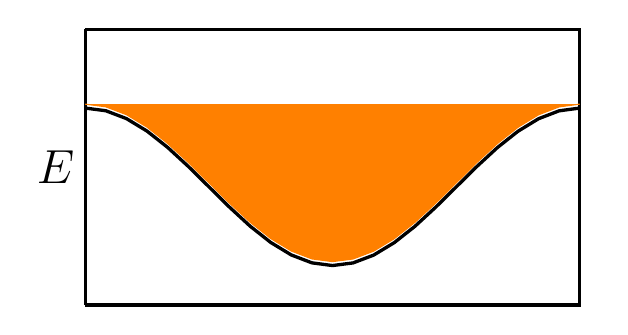
\begin{tikzpicture}[domain=0:6.28]
      \draw[very thick] (0, -2.5) -- (0,1) node[left, midway] {\LARGE $E$} ;
      \draw[very thick] (0, 1)-- (6.28,1) -- (6.28, -2.5) -- (0, -2.5);
      \draw[color=black, very thick] plot (\x,{-1+cos(\x r)}) node[right] {};
      \draw[color=orange, fill] plot (\x,{-0.95+cos(\x r)}) {};
  \end{tikzpicture}
  
            }
        \caption{Band Insulator}
        \end{figure}
    \end{column}
    \begin{column}[T]{.6\textwidth}
        \begin{figure}[h]
            \scalebox{1.4}{
            \input{diagrams/aklt_bare.tex}
            }
            \caption{Heisenberg AF Spin-1 chain}
        \end{figure}
    \end{column}
\end{columns}
\end{frame}
%\subsection{Band Insulators}
\newcommand{\kk}{\mathbf{k}}
\begin{frame}{Free Fermion Band Insulators}
\vskip-1.5cm
\begin{columns}[T]
\begin{column}[T]{0.65\textwidth}
\bi 
\item Crystaline, 0T insulators \\(including semiconductors)
%A good source of examples - column IV of periodic table, such as C, or in combination with column VI 
%(Columns I-III prefer to donate their valence electrons and form ionic bonds or metals)
%Microscopics are described well by
\item Tight-binding Hamiltonian 
$$
\mathcal{H}_{FF} =  \sum\limits_{<ij>}\sum\limits_{\alpha, \beta}-t_{\alpha, \beta} c^{\alpha \dagger}_{i} c_{j}^{\beta} - \mu \sum\limits_{i, \alpha} N_{i}^{\alpha} 
$$
%Diagonalize in momentum space to produce band picture, completely fill some lowest number of bands
\item Bloch Wavefunctions
$
\ket{u^{\alpha}_{\kk}}
$
%Low energy physics can be described by the Dirac Hamiltonian, with an effective mass for electron-like excitations, which looks in 2d like
\item Massive Dirac Hamiltonian 
$$
\mathcal{H}_{D}(\kk) = \kk_x \sigma_x + \kk_y \sigma_y + m_*\sigma_z
$$
%Describing a single conduction and valence band with a gap to pair production of quasi-electron+quasi-hole
\item Atomic-insulating like Wannier basis
%From Fourier transforming the Block wavefunctions
\ei 
\end{column}

\begin{column}[T]{0.35\textwidth}
\vskip3cm
\only<1>{
    \begin{figure}
        \includegraphics[width=\linewidth]{diagrams/GaNcrystal.jpg}
        \caption{Semiconductor GaN}
    \end{figure}
}    
\only<2>{
    \begin{figure}
        \includegraphics[width=\linewidth]{diagrams/GaNcrystal.jpg}
        \caption{Band Theory}
    \end{figure}
}
\only<3>{
    \begin{figure}
        \includegraphics[width=\linewidth]{diagrams/GaNcrystal.jpg}
        \caption{Dirac Band Theory}
    \end{figure}
}
\only<4>{
    \begin{figure}
        \includegraphics[width=\linewidth]{diagrams/GaNcrystal.jpg}
        \caption{Wannier Function}
    \end{figure}
}
\end{column}
\end{columns}
\end{frame}
\begin{frame}{Free Fermion Band Insulators}
\vskip-1.5cm
\begin{columns}[T]
\begin{column}[T]{0.65\textwidth}
\end{column}
\end{columns}
\end{frame}
\begin{frame}{$\mathcal{T}$-Symmetric Honeycomb Band Insulators}
\vskip-1.5cm
\begin{columns}
\begin{column}[T]{0.65\textwidth}
%Famously
From considerations of graphene, a tight-binding honeycomb lattice model of fermions:

\bi
\item A spinless fermion has protected Dirac points
\bi
\item with $\mathcal{I}$ and $\mathcal{T}$ symmetry
\item NO featureless insulators at filling 1 on the honeycomb lattice with $\mathcal{T}$
%One way to say it: T guarantees m = m' where m and m' are the effective masses at the special momenta labeled K and K'
% On the otherhand, I guarantees m=-m' and with T broken gives a chern number \pm1. 
\ei 
\item<2-> Breaking  $\mathcal{T}$ leads to non-zero Chern number - $\mathbb{Z}$ invariant, QAHE 
%Haldane proposed using complex hopping amplitudes to do this in 1988 instead of a static magnetic field, QAHE -IQHE without net magnetic flux

%This situation can be exploited to make something new, by taking two copies.
\item<3-> Spinful fermions with spin-orbit couplings have two bands, with Chern numbers $\pm 1$.
%Net chern number and qhconductance is zero but there is quantum spin hall current
%Charlie Kane 2004
%2d topological insulator, edge is a kramers doublet in general
\item<3-> $\mathbb{Z}_2$ topological invariant 
\vskip-0.3cm
\ei
\end{column}
\begin{column}[T]{0.35\textwidth}
\only<1>{
    \begin{figure}
        \includegraphics[width=\linewidth]{diagrams/grapheneband2.jpg}
        \caption{Dirac Points}
    \end{figure}
    \vskip-2cm
        \begin{figure}
        \includegraphics[width=\linewidth]{diagrams/kpoint.png}
        \caption{Brillouin Zone}
    \end{figure}
}
\only<2->{
\begin{figure}
\includegraphics[width=\linewidth]{diagrams/helical_edge.png}
\caption{Helical Edge \footnotemark}
\end{figure}
\vskip-0.5cm
\bi 
\item $\mathcal{T}$-symmetric quantum spin-hall insulator.
%spin-hall conductance is non-zero
%edges can be gapped out by breaking T
\ei }
\end{column}
\end{columns}
\footnotetext[2]{
\citep{Hasan2010-fq}} 
\end{frame}
\begin{frame}{Free Fermion Edge Classification}
\vskip-1.5cm
\only<1>{
By partitioning the wavefunction, we can glimpse the edge
\begin{columns}[T]
\begin{column}{0.5\textwidth}
\begin{figure}
\includegraphics[width=\linewidth]{diagrams/QSH.png}
\caption{Top: Physical spectrum with boundary.
Bottom: 'Single particle entanglement spectrum'}
\end{figure}
\end{column}
\begin{column}{0.5\textwidth}
\bi
\item $G_{ij} = \ev{c^{\dagger}_i c_j}$ 
%\item Determines free fermion state
%\item Eigenvalues are 1, 0
\item $G^L_{ij}$ is G restricted to left half of cylinder
\item Spectrum of $G^L$ shown.
\item 'Gapless entanglement mode' protected by $\mathcal{T}$

\item Bulk wavefunction E.S. shown to capture edge physics
\item Bulk wavefunction shown to be distinct from atomic insulator
\ei 

\end{column}
\end{columns}
}
\only<2>{
    Results for free fermions without lattice symmetries:
    \begin{figure}
    \includegraphics[width=\linewidth]{diagrams/AZ.png}
    \caption{Free-fermion classification (ten-fold way) for $       \mathcal{T}, \mathcal{C}$} 
    \end{figure}
    \footnotetext[5]{
    \citep{Ryu2009-qc}} 
%These invariants aren't always very physical, and while they distinguish free fermion Hamiltonians, they aren't guaranteed to stick around when you add interactions.

% Most of the invariants are only well defined in the presence of some additional symmetry

% There is an big table of free-fermion classification called the 10 fold way for time-reversal and charge conjugation symmetry, and a bigger table when you include lattice symmetries (Topological Crystalline Insulators)
}


\end{frame}
\begin{frame}{Motivating Questions}
\vskip-1.5cm
%We want to classify and understand all featureless insulators, 
%but thats a big undertaking so lets break that question down into some smaller questions.


\begin{block}{Existence}
Fix a lattice $\Lambda$, symmetry group $G$, and integer filling number $m$

Do there exist any featureless insulators at all?
\bi 
\item Find \textbf{obstruction} to existence
\item or \textbf{construct} a reference featureless insulator
\ei 
%The Lieb-Schultz-Mattis theorem gives one such constraint - m must be an integer. Is that the only constraint? Can you prove it by constructing featureless insulators for every m? You might try to construct one and realize that there are additional obstructions that you haven't thought of yet, which would allow you to extend the LSM theorem.
\end{block}

\begin{block}{Characterization}
Given a quantum wavefunction, is it a featureless insulator? Is it distinguishable from atomic insulator in the presence of a symmetry group $G$? What is $G$?

\bi
\item Show non-trivial protected physical or entanglement edge modes 
\item Find a topological invariant that distinguishes it
\ei 
\end{block}
\end{frame}
%\subsection{Bosonic Mott Insulators}
\begin{frame}{Bosonic Mott Insulators}
\vskip-1.5cm

\only<1>{
        \begin{figure}
        \centering
        \includegraphics[width=\linewidth]{diagrams/SuperfluidStates.jpg}
        \caption{Mott insulator with cold atoms in optical lattice\footnotemark}
        \end{figure}
        }
\begin{block}{Bose-Hubbard model}
\vskip-0.3cm
$$
H_{BH} = -J \sum\limits_{<ij>} b^{\dagger}_i b_j - \mu \sum\limits_i N_i + \frac12 V \sum\limits_i N_i (N_i-1)
$$
\end{block}
\only<2->{
\begin{columns}[T]
    \begin{column}[T]{.4\textwidth}
        \vskip-1.2cm

        \only<2>{
        \begin{figure}
        \centering
        \includegraphics[width=\linewidth]{diagrams/bosehubbard2.png}
        \end{figure}
        }
    \end{column}
    \begin{column}[T]{.6\textwidth}
    \vskip-0.7cm
    \bi
    \item Form an atomic insulator with N bosons to minimize $-\mu N + VN(N-1)/2$
    %Particles and holes have a cost based on this function
    %particle cost goes to zero at transition between fillings
    \item Gap to particle/hole excitations
    %Kinetic energy causes some local density fluctuations, but not much else
    \item Bosons free to hop will instantly condense into superfluid with any $J$
    %Must have interactions, and in cold atoms
    %Deep optical lattice wells to keep $J$ small enough
    \item Number conserving - so no superfluid phase coherence
    %\item Unlike free-fermions, not obvious how to construct fractional site filling insulators
    %\item Tensor network states give us access to needed construction and to interacting invariants.
    %\note{LSM inspired invariants}
    \ei
    \end{column}
\end{columns}
}
\only<1>{
\footnotetext[3]{\citep{Greiner2002-ay}}
}
\only<2>{
\footnotetext[4]{\citep{Fisher1989-ou}}
}
\end{frame}

%\subsection{Honeycomb Bosonic Mott Insulators?}
\begin{frame}{Honeycomb Bosonic Mott Insulators}
\vskip-1.5cm
Does there exist a featureless bosonic insulator with filling m=1 on the honeycomb?
\only<1>{
\begin{figure}
\scalebox{1}{
%
% x=3*(minimum size)/2
% y=\sqrt{3/4}*(minimum size)/2
%

%http://tex.stackexchange.com/questions/6019/drawing-hexagons
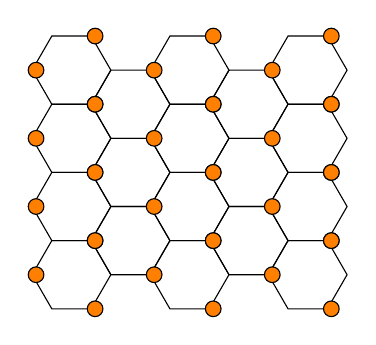
\begin{tikzpicture}[x=7.5mm,y=4.33mm]
  % some styles
  \tikzset{
    box/.style={
      regular polygon,
      regular polygon sides=6,
      minimum size=10mm,
      inner sep=0mm,
      outer sep=0mm,
      rotate=0,
    draw
    }
  }
 \tikzset{boson/.style={circle=1pt,draw=black!100,fill=orange!100,inner sep=2pt}}

\foreach \i in {0,...,2} 
    \foreach \j in {0,...,3} {
            \node[box] at (2*\i,2*\j) {};
        }
\foreach \i in {0,...,1} 
    \foreach \j in {0,...,2} {
   	   \node[box] at (2*\i+1,2*\j+1) {};   
        }
\foreach \i in {0,...,2} 
    \foreach \j in {0,...,3} {
            \node[boson] at (2*\i-0.6,2*\j) {};
           % \node[boson] at (2*\i+0.6,2*\j) {};
           % \node[boson] at (2*\i-0.4,2*\j-1) {};
           % \node[boson] at (2*\i-0.4,2*\j+1) {};
             \node[boson] at (2*\i+0.4,2*\j+1) {};
              \node[boson] at (2*\i+0.4,2*\j-1) {};
        }
%\foreach \i in {0,...,1} 
  %  \foreach \j in {0,...,2} {
%	\node[boson] at (2*\i+1-0.6,2*\j+1) {}; 
%	\node[boson] at (2*\i+1+0.6,2*\j+1) {};   
   %   }
      
\end{tikzpicture}

}
\caption{Breaks point group symmetry $D_6$ to $D_3$}
\end{figure}}
\only<2>{
\begin{figure}
\scalebox{1}{
% y=\sqrt{3/4}*(minimum size)/2
%

%http://tex.stackexchange.com/questions/6019/drawing-hexagons
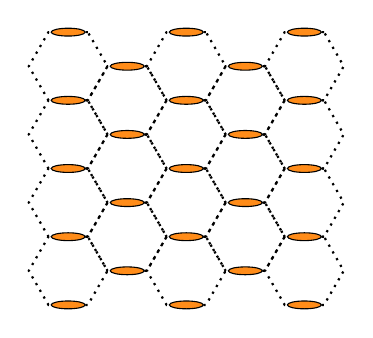
\begin{tikzpicture}[x=7.5mm,y=4.33mm]
  % some styles
  \tikzset{
    box/.style={
      regular polygon,
      regular polygon sides=6,
      minimum size=10mm,
      inner sep=0mm,
      outer sep=0mm,
      rotate=0,
      dotted,
      thick,
      black,
      draw
    }
  }
 \tikzset{boson/.style={circle=1pt,draw=black!100,fill=orange!100,inner sep=2pt}}
  \tikzset{dimer/.style={ellipse=1pt,draw=black!100,fill=orange!90,inner sep=2pt}}
    \tikzset{thindimer/.style={ellipse=1pt,draw=black!100,fill=orange!90,inner sep=1pt}}

\foreach \i in {0,...,2} 
    \foreach \j in {0,...,3} {
            \node[box] at (2*\i,2*\j) {};
        }
\foreach \i in {0,...,1} 
    \foreach \j in {0,...,2} {
   	   \node[box] at (2*\i+1,2*\j+1) {};   
        }

 \foreach \i in {-1,...,2} 
     \foreach \j in {-1,...,2} 
     {
     \pgfmathtruncatemacro{\xa}{2*\i + 1*\j}
     \pgfmathtruncatemacro{\ya}{3*\j}
      \pgfmathtruncatemacro{\xb}{2*\i + 1*\j+1}
     \pgfmathtruncatemacro{\yb}{3*\j+1}
      \pgfmathtruncatemacro{\xc}{2*\i + 1*\j}
     \pgfmathtruncatemacro{\yc}{3*\j+2}
    
    \ifnum -1<\xa \ifnum \xa<5
     \ifnum\ya<7\ifnum-1<\ya 
	% \node[thindimer, rotate=120] at (\x-1/2,\y-1/2) {$\,\,\,\,$};     
     %\node[thindimer, rotate=120] at (\x+1/2,\y+1/2) {$\,\,\,\,$};
     %\node[thindimer, rotate=60] at (\x-1/2,\y+1/2) {$\,\,\,\,$};
       %\node[thindimer, rotate=60] at (\x+1/2,\y-1/2) {$\,\,\,\,$};
     \node[thindimer, rotate=0] at (\xa,\ya-1) {$\,\,\,\,$};
      \node[thindimer, rotate=0] at (\xa,\ya+1) {$\,\,\,\,$};
     \fi \fi\fi\fi
     
      \ifnum -1<\xc\ifnum \xc<5
     \ifnum \yc<7 \ifnum -2<\yc
       \node[thindimer, rotate=0] at (\xc,\yc+1) {$\,\,\,\,$};
       \fi\fi\fi \fi 
     }

\end{tikzpicture}
}
\caption{Breaks rotational symmetry}
\end{figure}}
\only<3>{
\begin{figure}
\scalebox{1}{
%
% x=3*(minimum size)/2
% y=\sqrt{3/4}*(minimum size)/2
%

%http://tex.stackexchange.com/questions/6019/drawing-hexagons
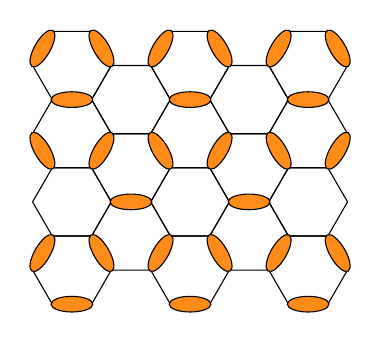
\begin{tikzpicture}[x=7.5mm,y=4.33mm]
  % some styles
  \tikzset{
    box/.style={
      regular polygon,
      regular polygon sides=6,
      minimum size=10mm,
      inner sep=0mm,
      outer sep=0mm,
      rotate=0,
    draw
    }
  }
 \tikzset{boson/.style={circle=1pt,draw=black!100,fill=orange!100,inner sep=2pt}}
  \tikzset{dimer/.style={ellipse=1pt,draw=black!100,fill=orange!90,inner sep=2pt}}

\foreach \i in {0,...,2} 
    \foreach \j in {0,...,3} {
            \node[box] at (2*\i,2*\j) {};
        }
\foreach \i in {0,...,1} 
    \foreach \j in {0,...,2} {
   	   \node[box] at (2*\i+1,2*\j+1) {};   
        }
% \foreach \i in {0,...,2} 
%     \foreach \j in {0,...,3} {
%     	  %\node[boson] at (2*\i-0.4,2*\j+1) {}; %TL of A hexagon
%          %\node[boson] at (2*\i+0.6,2*\j) {}; %R of A hexagon
%          %\node[boson] at (2*\i-0.4,2*\j-1) {}; %BL of A hexagon
% 
%          %\node[boson] at (2*\i-0.6,2*\j) {}; %L of  A hexagon
%          %\node[boson] at (2*\i+0.4,2*\j+1) {}; %TR of A hexagon
%          %\node[boson] at (2*\i+0.4,2*\j-1) {}; %BR of A hexagon
%         }
% \foreach \i in {0,...,1} 
%     \foreach \j in {0,...,2} {
% %	\node[boson] at (2*\i+1-0.6,2*\j+1) {}; %L of B hexagon
% %	\node[boson] at (2*\i+1+0.6,2*\j+1) {};   %R of B hexagon
%       }
 \foreach \i in {-1,...,2} 
     \foreach \j in {0,...,2} 
     {
     \pgfmathtruncatemacro{\x}{2*\i + 1*\j}
     \pgfmathtruncatemacro{\y}{3*\j}
     \ifnum
     -1<\x
     \ifnum
     \x<5
     \ifnum
     \y<7
     \ifnum
     -1<\y     
     \node[dimer, rotate=120] at (\x+1/2,\y+1/2) {$\,\,\,\,$};
     \node[dimer, rotate=60] at (\x-1/2,\y+1/2) {$\,\,\,\,$};
     \node[dimer, rotate=0] at (\x,\y-1) {$\,\,\,\,$};
     \fi
     \fi
     \fi
     \fi
     %\node[boson] at (\x, \y) {}; 
     }
    \node[dimer, rotate=120] at (0-1/2,3+1/2) {$\,\,\,\,$};
    \node[dimer, rotate=60] at (5-1/2,3+1/2) {$\,\,\,\,$};
      
\end{tikzpicture}
}
\caption{Breaks translationally symmetry, unit cell is 3 times larger}
\end{figure}}
\end{frame}
\begin{frame}[c]{Can we use `band bosons`?}
\vskip-1.5cm
\only<1>{
Band fermions have atomic insulator picture using Wannier functions.

$$W^{\alpha}_R(x) = \int_{B.Z.} d\kk e^{-iR\cdot \kk} \psi^{\alpha}_{\kk}(x)$$

$$d_R^{\alpha \dagger} = \sum\limits_x W^{\alpha}_R(x)c_x^{\dagger}$$ 

$$\ket{\psi} = \prod\limits_R d_R^{\alpha \dagger} \ket{\mathbf{0}} $$

Wannier functions are not unique and often don't respect lattice symmetries depending on choice of phase for original basis functions. 
\\\vspace{1em}
But the resulting 'Slater determinant' wavefunction is symmetric regardless. 
%due to antisymmetrization
%individual wannier functions are not eigenstates unless the band is perfectly flat.
%This picture breaks down when the chern number of a band is not zero, or if bands touch.
}
% A band boson is defined in analogy to this slater determinant wave
\only<2>{
\begin{block}{`Band bosons' a.k.a. Boson Permanent}
{A boson permanent wavefunction created from filling an orbital $\phi_{R+x}$ for each unit cell $R$ with a boson}
\end{block}
Analogous to the Slater determinant for fermions except:
%with a few key differences:
\bi 
\item $\ket{\psi}$ respects lattice symmetries only if $\phi$ does
%Boson permanent wavefunction won't respect lattice symmetries unless orbitals filled do.
\item $H$ needs repulsive interactions to stop Bose condensation
\bi 
\item e.g. $H_{BH}$ with $$d^{\dagger}_R = \sum\limits_i \phi_i b^{\dagger}_i$$
\ei
%use bose-hubbard repulsion
\item Orbitals will need to be localized and orthogonal for $H_{BH}$ to be a parent Hamiltonian
\ei 

%If we could find symmetric, orthogonal, localized orbitals, we can try fill them with bosons to make a 'band' boson featureless insulator with a nice parent Hamiltonian.
%Say by analyzing the fermion tightbinding model 
%Can do this on Kagome but not on honeycomb: the symmetry protection of the band touching is an obstruction
}
\end{frame}
\newcommand{\hexa}{}
\begin{frame}[t]{Honeycomb Mott Insulators}
\framesubtitle{Proposed Wavefunction}
\vskip-1cm
Key insight\footnotemark: 'Center of charge' must lie at symmetric point

%For 1 boson/unit cell
%Similar idea called 'polarization' plays a part in the classifcation of Topological Crystalline Insulators
%Its a berry phase computed from band wavefunctions, determines a point in the unit cell
%If there is no such point in the lattice, its called non-symmorphic and you can't (proof rigorized in same way as LSM, flux threading) find a featureless insulator  
$$
\ket{\psi} = \prod\limits_{\varhexagon} \left(\sum\limits_{i \in \varhexagon} b^{\dagger}_i \right) \ket{\mathbf{0}}
$$
\only<1>{
\begin{figure}[h]
\scalebox{1}{
\input{diagrams/fbi1.tex}
}
\end{figure}
}

\only<2>{
\begin{figure}[h]
\scalebox{1}{
\input{diagrams/fbi2.tex}
}
\end{figure}
}

\only<3>{
\begin{figure}[h]
\scalebox{1}{
\input{diagrams/fbi3.tex}
}
\end{figure}
}

\only<4->{
\begin{figure}[h]
\scalebox{1}{
\documentclass[twocolumn,english,prb,showpacs]{revtex4-1}
\usepackage[colorlinks=true,urlcolor=blue,citecolor=blue,linkcolor=blue]{hyperref}
\usepackage[T1]{fontenc}
\usepackage[latin9]{inputenc}
\usepackage{amssymb}
\usepackage{graphicx}
\usepackage{amsmath,color}
\usepackage{mathrsfs}
\usepackage{float}
\usepackage{indentfirst}
\usepackage{babel}
\usepackage[sort&compress]{natbib}
\usepackage{color}

\newcommand{\bela}[1]{[\emph{\color{blue}{Bela: #1}}]}
\newcommand{\brayden}[1]{[\emph{\color{red}{Brayden: #1}}]}
\newcommand{\eqnref}[1]{Eq.~(\ref{#1})}

%\makeatletter

\begin{document}

\title{Not so featureless after all: symmetry protected order in an interacting boson state}

\author{Brayden Ware}

\author{Itamar}
\author{Sid}

\author{Bela Bauer}
\affiliation{Station Q, Microsoft Research, Santa Barbara, CA 93106-6105, USA}

\begin{abstract}
...
\end{abstract}
\maketitle

\section{Introduction}


\section{Conclusions}

\acknowledgements


\bibliography{fbi}


\end{document}

}
\end{figure}

%No valid Wannier functions, so we sacrifice 
Overlapping orbitals NOT orthogonal
%Or boson operators don't commute
}
\only<1-3>{\footnotetext[3]{\citep{Kimchi2012-lr}}}
\end{frame}
\begin{frame}{Goals for Honeycomb Mott Insulator}
\vskip-1.5cm
\bi 
\item Build a tensor network representation for doing computations
\item <1-> Verify that no spontaneous symmetry breaking occurs
%We'll do this by computing correlation functions on a cylinder geometry combined with scaling analysis in the circumference

\only<1>{
\begin{figure}
\includegraphics[width=6cm]{diagrams/kimchicorr.png}
\caption{Exponentially decaying rotationally symmetric correlations computed using Monte Carlo sampling, \citep{Kimchi2012-lr}}
\end{figure}
}

\only<2->{
\begin{figure}
\includegraphics[width=6cm]{diagrams/Zig.png}
\end{figure}

\item<3-> Rule out topological order

\item<4-> Compute entanglement spectrum to check for nontrivial entanglement
\item<5-> Understand the role of symmetries in protecting entanglement in interacting quasi-1D and 2D theories
\item<6-> Find distinguishing topological invariant and/or physical signatures
\item<7-> Find a parent Hamiltonian 
%then you can do things like perturb hamiltonian to show that it is a stable phase if certain symmetries are kept, and drive phase transitions to lattice SB insulators or superfluids.
% also you can dope it and make a superfluid with some properties.

}
\ei 
\end{frame}

\section{Entanglement}
\begin{frame}{What is entanglement?}
\vskip-1.5cm
 When a wavefunction in a product Hilbert space cannot be written as a product state, it is \textbf{entangled}.
\only<1-2>{ 
\begin{block}{}
\begin{columns}[T]
    \begin{column}{.5\textwidth}
    $$
    \ket{\psi} = \ket{\psi_L} \otimes \ket{\psi_R} ?
    $$
    \end{column}
    \begin{column}[T]{.5\textwidth}
        \only<1>{
        \note{A state in a product Hilbert space is a tensor}
        \vskip-1.5cm
        \begin{figure}
        \scalebox{0.8}
        {
        %!TEX root = ../thesis.tex

%\beginpgfgraphicnamed{diagrams}
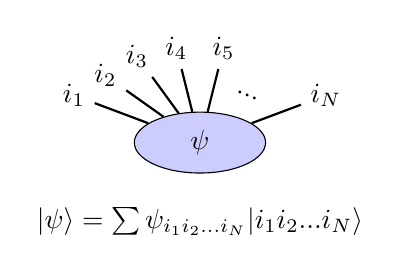
\begin{tikzpicture}[node distance=0.4cm]
%\tikzset{ellip/.style={ellipse (3 and 1), fill=blue!20, draw=black, inner sep=4pt}}
\tikzset{det/.style={circle=2pt,fill=blue!20,draw=black,inner sep=4pt}}
%\draw (1,1) ellipse [x radius=1cm,y radius=.5cm];
\node[ellipse, rotate=0, draw, fill=blue!20] (t) at (0,0) {\, \, $\psi$ \, \,};
\node (t1) at (-1.6, 0.6) {$i_1$};
\node (t2) at (-1.2 ,0.85) {$i_2$};
\node (t3) at (-0.8,1.1) {$i_3$};
\node (t4) at (-0.3,1.2) {$i_4$};
\node (t5) at (0.3, 1.2) {$i_5$};
\node (tN) at (1.6, 0.6) {$i_N$};
\node[rotate=-20] (d) at (0.6, 0.6) {...};
%\node (tl) at (1,-0.4) {$l$};
\draw[thick] (t1) -- (t);
\draw[thick] (t2) -- (t);
\draw[thick] (t3) -- (t);
\draw[thick] (t4) -- (t);
\draw[thick] (t5) -- (t);

\draw[thick] (tN) -- (t);
%\node[in of=t] {$\psi$};
\node (p) at (0,-1) {$|\psi \rangle = \sum \psi_{i_1 i_2 ... i_N} \vert i_1 i_2 ... i_N \rangle$};


%\draw  (-0.8,2.4) node (v1) {} ellipse (1.2 and 0.4);
%\draw  (v1) ellipse (0 and 0);
\end{tikzpicture}
%\endpgfgraphicnamed
        }
        \end{figure}
        }
        \only<2>{
        \begin{figure}
        \vskip-1cm
        \scalebox{1}
        {
        \input{diagrams/productstate.tex}
        }
        \note{going from the RHS to LHS - performing that sum - is tensor contraction. going from LHS to RHS is finding a decomposition of the tensor, and is not a unique process.}
        \end{figure}
        }
    \end{column}
\end{columns}
\end{block}
}
\only<3->{
\begin{block}{}
\begin{columns}[T]
    \begin{column}[T]{.5\textwidth}
    $$
    \ket{\psi} = \sum\limits_i \ket{\psi^i_L} \otimes \ket{\psi^i_R}
    $$
    \end{column}
    \begin{column}[T]{.5\textwidth}
        \begin{figure}
        \vskip-1cm
        \scalebox{1}
        {
        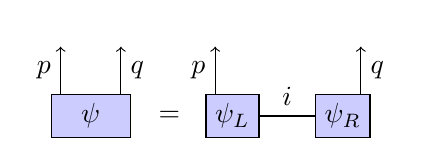
\begin{tikzpicture}[node distance=0.6cm]
\node[side, minimum width=1cm] (psi) at (0,0) {$\psi$};
\node[above=of psi.north west, anchor=south west] (p) {};
\node[above=of psi.north east, anchor=south east] (q) {};
 \draw[->] (psi.north -| p) -- node[left] {$p$} (p);
 \draw[->] (psi.north -| q) -- node[right] {$q$} (q);
 
 \node at (1, 0) {=};
 
 \node[side] (psiL) at (1.8,0) {$\psi_L$};
  \node[side] (psiR) at (3.2,0) {$\psi_R$};
\node[above=of psiL.north west, anchor=south west] (pL) {};
\node[above=of psiR.north east, anchor=south east] (qR) {};
 \draw[->] (psiL.north -| pL) -- node[left] {$p$} (pL);
 \draw[->] (psiR.north -| qR) -- node[right] {$q$} (qR);
 \draw[thick] (psiL) -- node[above] {$i$}(psiR);
 
\end{tikzpicture}

% http://hugoideler.com/2013/01/tikz-node-positioning/
% \begin{tikzpicture}[
  % every node/.style={draw, minimum size=1cm, thick, fill=white, rounded corners},
  % hi/.style={fill=red!50},
  % low/.style={fill=blue!50},
% ]
  % \node[low, minimum width=5cm] (basis) {};
  % \node[hi, above=of basis.north west, anchor=south west] (a) {A};
  % \node[hi, above=of basis] (b) {B};
  % \node[hi, above=of basis.north east, anchor=south east] (c) {C};

  % \draw[->] (basis.north -| a) -- (a);
  % \draw[->] (basis) -- (b);
  % \draw[->] (basis.north -| c) -- (c);

  % \end{tikzpicture}
        }
        \end{figure}
    \end{column}
\end{columns}
\end{block}
}
\only<3>{
\begin{block}{}
\vskip-0.5cm
Calculate reduced density matrices
\begin{columns}[T]
    \begin{column}[T]{.5\textwidth}
    $$
    \rho_L = Tr_R \ket{\psi} \bra{\psi} 
    $$
    
    \hskip0.3cm Diagonalize 
    
    $$
    \hskip0.1cm
    \rho_L = \sum\limits_{\alpha} \rho_{\alpha} \ket{\psi_L^{\alpha}} \bra{\psi_L^{\alpha}} 
    $$
    \end{column}
    \begin{column}[T]{.5\textwidth}
        \begin{figure}
        \vskip-0.5cm
        \scalebox{1}
        {
        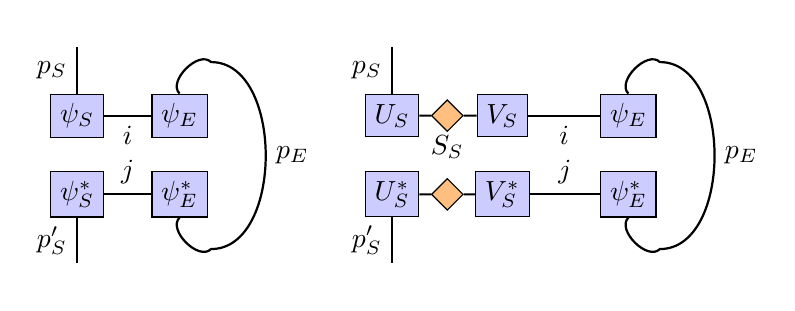
\begin{tikzpicture}[node distance=0.6cm]
\node[side] (kL) at (0,0) {$\psi_S$};
\node[side] (kR) at (1.3, 0) {$\psi_E$};
\draw[thick] (kL) -- node[below] {$i$} (kR);
\node (kLp) at (0, 1) {};
\draw[thick] (kL) -- node[left] {$p_S$} (kLp);

\node[side] (bL) at (0,-1) {$\psi_S^*$};
\node[side] (bR) at (1.3, -1) {$\psi_E^*$};
\draw[thick] (bL) -- node[above] {$j$} (bR);
\node (bLp) at (0, -2) {};
\draw[thick] (bL) -- node[left] {$p'_S$} (bLp);

\node (kRp) at ($(kR.north)+(0.4, 0.4)$) {};
\node (bRp) at ($(bR.south)+(0.4, -0.4)$) {};
\draw[thick] (kR.north) to [bend left= 90] (kRp.center) to  [bend left=90] node[right] {$p_E$}  (bRp.center) to [bend left=90] (bR.south);


\node[side] (UL) at (4, 0) {$U_S$};
\node[side] (VL) at (5.4, 0) {$V_S$};
\node[lambda] (SL) at (4.7, 0) {};
%\node[bel0w of=S] {$S_S$};

\draw[thick] (UL) -- (SL) -- (VL);
%\node[side] (kL) at (4,0) {$\psi_S$};
\node[side] (kR) at (7, 0) {$\psi_E$};
\draw[thick] (VL) -- node[below] {$i$} (kR);
\node (kLp) at (4, 1) {};
\draw[thick] (UL) -- node[left] {$p_S$} (kLp);


\node[side] (UdL) at (4, -1) {$U_S^*$};
\node[side] (VdL) at (5.4, -1) {$V_S^*$};
\node[lambda] (SdL) at (4.7, -1) {};
\node[above of=SdL] {$S_S$};

\draw[thick] (UdL) -- (SdL) -- (VdL);
\node[side] (bR) at (7, -1) {$\psi_E^*$};
\draw[thick] (VdL) -- node[above] {$j$} (bR);
\node (bLp) at (4, -2) {};
\draw[thick] (UdL) -- node[left] {$p'_S$} (bLp);

\node (kRp) at ($(kR.north)+(0.4, 0.4)$) {};
\node (bRp) at ($(bR.south)+(0.4, -0.4)$) {};
\draw[thick] (kR.north) to [bend left= 90] (kRp.center) to  [bend left=90] node[right] {$p_E$}  (bRp.center) to [bend left=90] (bR.south);


\end{tikzpicture}
        }
        \end{figure}
    \end{column}
\end{columns}
\end{block}
}
\only<4->{
\begin{block}{}
\vskip-0.5cm
Diagonalize and form the Schmidt decomposition
\note{Equivalent to SVD}
\note{Schmidt states are orthonormal}
\begin{columns}[T]
    \begin{column}[T]{.5\textwidth}
    $$
    \ket{\psi} = \sum\limits_{\alpha} \sqrt{\rho_{\alpha}} \ket{\psi^{\alpha}_L} \otimes \ket{\psi^{\alpha}_R}
    $$
    \end{column}
    \begin{column}[T]{.5\textwidth}
        \begin{figure}
        \vskip-0.5cm
        \scalebox{1}
        {
        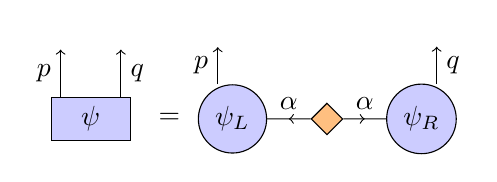
\begin{tikzpicture}[node distance=0.6cm]
\begin{scope}[decoration={
    markings,
    mark=at position 0.5 with {\arrow{>}}}
    ]
\node[side, minimum width=1cm] (psi) at (0,0) {$\psi$};
\node[above=of psi.north west, anchor=south west] (p) {};
\node[above=of psi.north east, anchor=south east] (q) {};
 \draw[->] (psi.north -| p) -- node[left] {$p$} (p);
 \draw[->] (psi.north -| q) -- node[right] {$q$} (q);
 
 \node at (1, 0) {=};
 
 \node[cside] (psiL) at (1.8,0) {$\psi_L$};
\node[lambda] (S) at (3, 0) {};
  \node[cside] (psiR) at (4.2,0) {$\psi_R$};
\node[above=of psiL.north west, anchor=south west] (pL) {};
\node[above=of psiR.north east, anchor=south east] (qR) {};
 \draw[->] (psiL.north -| pL) -- node[left] {$p$} (pL);
 \draw[->] (psiR.north -| qR) -- node[right] {$q$} (qR);
 \draw[-, postaction={decorate}] (S) -- node[above]{$\alpha$}(psiL);
 \draw[-, postaction={decorate}] (S) -- node[above]{$\alpha$}(psiR);
 
\end{scope}
\end{tikzpicture}
        }
        \end{figure}
    \end{column}
\end{columns}
\end{block}
\begin{block}{}
\vskip-0.5cm
\only<4>{
Quantitative measures of entanglement - rank
 $$
 S^0_A = \sum\limits_{\alpha} \rho_{\alpha}^0 = \#\{\rho_{\alpha} \ne 0\}
 $$
 \note{bond dimension}
 }
\only<5>{
Quantitative measures of entanglement - entropy
 $$
 S_A = -\sum\limits_{\alpha} \rho_{\alpha} \log{\rho_{\alpha} }
 $$
 \note{Capture MOST of the entanglement by using the largest eigenvalues, gives best possible approximation for a given bond dimension} 
 }
\end{block}
}

\end{frame}


\begin{frame}{Entanglement Entropy Area Law} 
\vskip-1.5cm
Ground states of gapped quantum Hamiltonians satisfy an area law: 
$$
S_V \lesssim d \cdot (\partial V) - \gamma
$$

$\gamma$ is universal and detects presence of topological order

In 1D:

\begin{columns}[T]
    \begin{column}[T]{.33\textwidth}
        \begin{figure}[h]
            %\captionsetup{justification=right}
            \centering
            $$S(x) \lesssim d $$
            \scalebox{0.45}{
             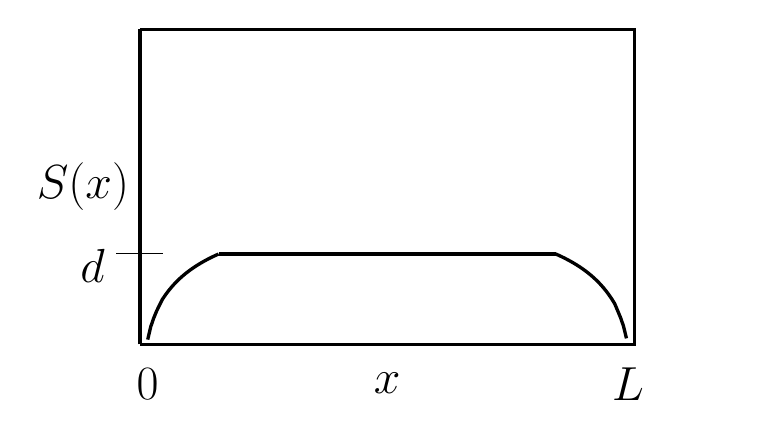
\begin{tikzpicture}[domain=0.1:6.18]
      \draw[very thick] (0, 0) -- (0,4) node[left, midway] {\LARGE $S(x)$} ;
     \node[] at (7.5, 2) {$$};
      \node[] at (3.14, -0.5){\LARGE $x$};
      \node[] at (-0.6, 1){\LARGE $d$};
      \draw[] (-0.3, 1.15) -- (0.3, 1.15);
       \node[] at (0.1, -0.5){\LARGE $0$};
       \node[] at (6.2, -0.5){\LARGE $L$};
      % \draw[thick] (0, 3.05) -- (3.14, 3.05);
      \draw[very thick] (0, 4)-- (6.28,4) -- (6.28, 0) -- (0, 0);
      \draw[color=black, very thick, domain=0.1:1] plot (\x,{1.5+1/3*log2(sin(\x/2 r))}) node[right] {};
	\draw[color=black, very thick, domain=1:5.28] plot (\x,{1.5+1/3*log2(sin(1/2 r))}) node[right] {};
	\draw[color=black, very thick, domain=5.28:6.18] plot (\x,{1.5+1/3*log2(sin(\x/2 r))}) node[right] {};
\end{tikzpicture}
            }
            \caption{Gapped ground state}
        \end{figure}
    \end{column}
    \begin{column}[T]{.33\textwidth}
            \begin{figure}[h]
            %\captionsetup{justification=right}
            \centering
            $$S(x) \lesssim c \log{x}$$
            \scalebox{0.45}{
             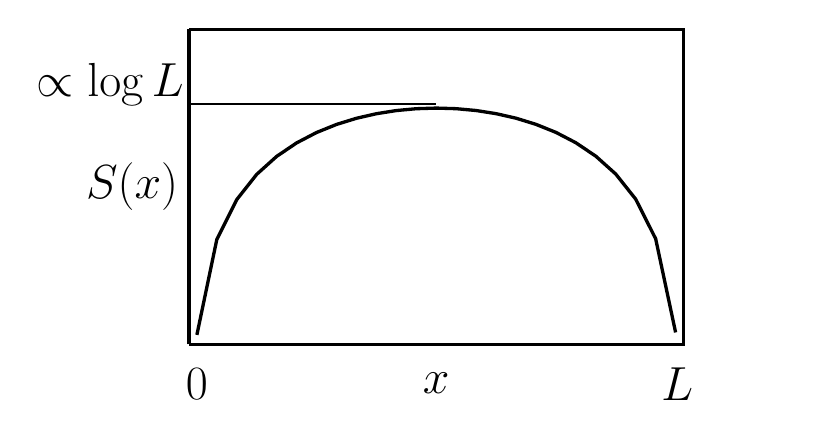
\begin{tikzpicture}[domain=0.1:6.18]
      \draw[very thick] (0, 0) -- (0,4) node[left, midway] {\LARGE $S(x)$} ;
       \node[] at (7.5, 2) {$$};
      \node[] at (3.14, -0.5){\LARGE $x$};
       \node[] at (-1, 3.3){\LARGE $\propto \log{L}$};
       \node[] at (0.1, -0.5){\LARGE $0$};
       \node[] at (6.2, -0.5){\LARGE $L$};
       \draw[thick] (0, 3.05) -- (3.14, 3.05);
      \draw[very thick] (0, 4)-- (6.28,4) -- (6.28, 0) -- (0, 0);
            \draw[color=black, very thick] plot (\x,{3+2/3*log2(sin(\x/2 r))}) node[right] {};
  \end{tikzpicture}
            }
            \caption{Gapless ground state}
        \end{figure}
    \end{column}
    \begin{column}[T]{.33\textwidth}
            \begin{figure}[h]
            %\captionsetup{justification=right}
            \centering
            $$S(x) \propto x $$
            \scalebox{0.45}{
             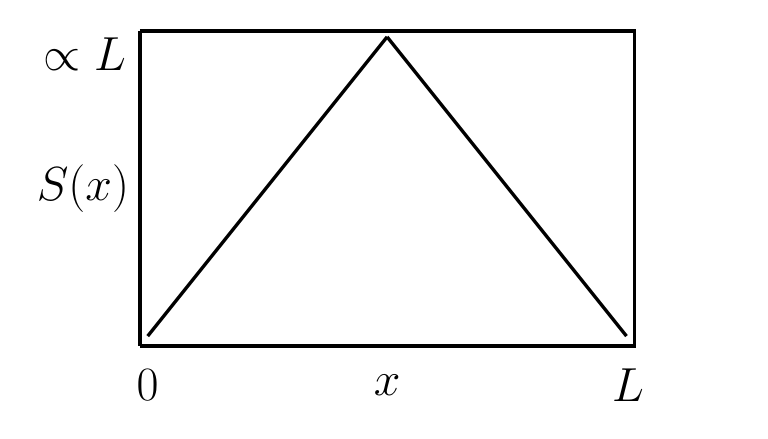
\begin{tikzpicture}[domain=0.1:6.18]
      \draw[very thick] (0, 0) -- (0,4) node[left, midway] {\LARGE $S(x)$} ;
       \node[] at (7.5, 2) {$$};
      \node[] at (3.14, -0.5){\LARGE $x$};
      \node[] at (0.1, -0.5){\LARGE $0$};
      \node[] at (6.2, -0.5){\LARGE $L$};
      \node[] at (-0.7, 3.7){\LARGE $\propto L$};
      \draw[very thick] (0, 4)-- (6.28,4) -- (6.28, 0) -- (0, 0);
      \draw[color=black, very thick, domain=0.1:3.14] plot (\x,{1.25*\x}) node[right] {};
      \draw[color=black, very thick, domain=3.14:6.18] plot (\x,{1.25*(6.28 - \x)}) node[right] {};
  \end{tikzpicture}
            }
            \caption{Generic State}
        \end{figure}
    \end{column}
\end{columns}
\end{frame}
    
\begin{frame}{Symmetry Protected Topological Phases}
\vskip-1.5cm
\only<1>{
Entanglement measures the obstruction from writing a single wavefunction as an atomic insulator. Protected entanglement is entanglement that can't be removed by adiabatic changes in the Hamiltonian.

\begin{block}{SPT phase}
 A phase of matter that cannot be connected adiabatically to an atomic insulator, using $G$-symmetric Hamiltonians, is called a {\em symmetry protected topological} or SPT phase.
\end{block}

\bi
\item No symmetry group needed, then topological ordered - not SPT.
\item Featureless but feature featured edges.
\bi 
\item Physical or entanglement edge, when cut respects $G$
\item Look for these patterns in entanglement spectra!
\ei 
\ei 
}



\end{frame}


\begin{frame}{Haldane Phase of Spin-1 Chain}
\vskip-1.5cm
\only<1>{
\begin{figure}
\scalebox{2}{
            \begin{frame}{MPS Example: AKLT State}
\vskip-1.5cm
\begin{block}{Haldane Phase for Spin-1 chains $(j=1, m=0)$}
\vskip-0.8cm
$$
H_{AKLT} = \sum\limits_{i} J \vec{S}_i\cdot \vec{S}_{i+1} + J' (\vec{S}_i\cdot \vec{S}_{i+1})^2 + D (S^z_i)^2+BS^x
$$
\end{block}
\begin{columns}[T]
    \begin{column}[T]{.45\textwidth}
        \vskip-1.2cm
        \begin{figure}
        \centering
        \includegraphics[width=\columnwidth]{diagrams/aklt2.png}
        \end{figure}
    \end{column}
    \begin{column}[T]{.55\textwidth}
    \vskip-0.8cm
    Two distinct featureless insulators:
    \bi 
    \item Large-D phase
    \bi 
    \item Contains product state wavefunction $\ket{\psi} = \ket{000...}$ 
    \ei
    \item Haldane phase
    \bi 
    \item Contains AKLT wavefunction $\ket{\psi} = \Sigma\ket{+00-0+...}$
    \ei 
        \begin{figure}[h]
            \hspace{-2cm}
            \scalebox{1.2}{
            \begin{frame}{MPS Example: AKLT State}
\vskip-1.5cm
\begin{block}{Haldane Phase for Spin-1 chains $(j=1, m=0)$}
\vskip-0.8cm
$$
H_{AKLT} = \sum\limits_{i} J \vec{S}_i\cdot \vec{S}_{i+1} + J' (\vec{S}_i\cdot \vec{S}_{i+1})^2 + D (S^z_i)^2+BS^x
$$
\end{block}
\begin{columns}[T]
    \begin{column}[T]{.45\textwidth}
        \vskip-1.2cm
        \begin{figure}
        \centering
        \includegraphics[width=\columnwidth]{diagrams/aklt2.png}
        \end{figure}
    \end{column}
    \begin{column}[T]{.55\textwidth}
    \vskip-0.8cm
    Two distinct featureless insulators:
    \bi 
    \item Large-D phase
    \bi 
    \item Contains product state wavefunction $\ket{\psi} = \ket{000...}$ 
    \ei
    \item Haldane phase
    \bi 
    \item Contains AKLT wavefunction $\ket{\psi} = \Sigma\ket{+00-0+...}$
    \ei 
        \begin{figure}[h]
            \hspace{-2cm}
            \scalebox{1.2}{
            \input{diagrams/aklt.tex}
            }
        \end{figure}

    \ei
    \end{column}
\end{columns}

\end{frame}
            }
        \end{figure}

    \ei
    \end{column}
\end{columns}

\end{frame}
            }
\end{figure}
\begin{columns}[T]
\begin{column}[T]{.5\textwidth}
\vskip-1.5cm
\begin{figure}
\includegraphics[width=\columnwidth]{diagrams/aklt2.png}
\end{figure}
\end{column}
   \begin{column}[T]{.5\textwidth}
   \vskip-1cm
    \includegraphics[width=\columnwidth]{diagrams/akltEE.png}
    \end{column}
\end{columns}
}
Haldane phase distinguished by exact double degeneracy in entire  entanglement spectrum.

Plotted using $E_{\alpha} = -\log{\rho_{\alpha}}$ or $\rho = e^{-H}$
\end{frame}
\begin{frame}{2D SPT Example: Chern Insulator}
\vskip-1.5cm
\begin{columns}[T]
\begin{column}[T]{.7\textwidth}
\begin{figure}
\includegraphics[width=\columnwidth]{diagrams/freefermionEE.png}
\end{figure}
\end{column}
\begin{column}[T]{.3\textwidth}
\bi 
\item Start with 'single particle entanglement spectra' of restricted correlation matrix $C_{ij}$
\item Transform the eigenvalues using $\log{\frac{C}{1-C}}$
\item Fill up to 'zero'
\item Result: Entanglement spectra
\ei
\end{column} 
\end{columns}

\end{frame}

\section{Tensor Networks}
\begin{frame}{What is a matrix product state?}
\vskip-1.5cm
Matrix product states provide a parameterization of the space of wavefunctions of a 1D or quasi-1D system.
\only<1, 3->{
\begin{figure}[h]
    \centering
    \scalebox{1}{
    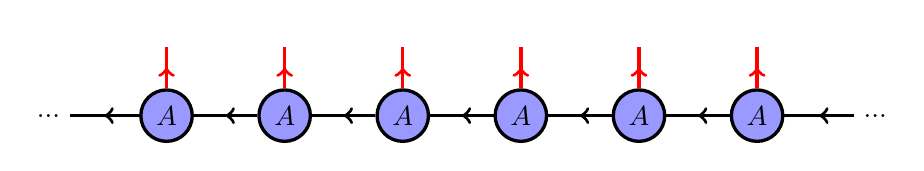
\begin{tikzpicture}[node distance=0.4cm]
\tikzset{gamma/.style={circle=2pt,draw=black!100, very thick, fill=blue!40, inner sep=3pt}}


\begin{scope}[decoration={
    markings,
    mark=at position 0.5 with {\arrow{>}}}
    ]

\foreach \i in {1,...,6} {
	\node[gamma] (G\i) at (1.5*\i,0) {$A$};
	\node (l\i) at ($ (G\i) + (0, 1) $) {$$};
	\draw[very thick, red!100, postaction={decorate}] (G\i) -- (l\i);
	%\node[below of=G\i] {$A$};
}

\foreach \i in {7} {
	\node[] (G\i) at (1.5*\i,0) {$...$};
    }  
    
\foreach \i / \j in {1/2,2/3,3/4,4/5,5/6, 6/7} {
	\draw[very thick, postaction={decorate}] (G\j) -- (G\i);
}
\node (b0) at (0, 0) {$...$};
\draw[very thick, postaction={decorate}] (G1) -- (b0);

\end{scope}
\end{tikzpicture}

    }
\end{figure}
\only<1>{
$$
\ket{\psi^{b_0 b_1}} = \sum\limits_{p_1 ... p_5}   \vbra{b_0} A^{p_1}_1 ... A^{p_5}_5 \vket{b_1}\ket{p_1 ... p_5} 
$$
}
Coefficients of the wavefunction are calculated via a product of matrices, one per site. The matrix at each site depends on the physical state at that site.
}

\only<2>{
\begin{figure}[h]
    \centering
    \scalebox{1}{
    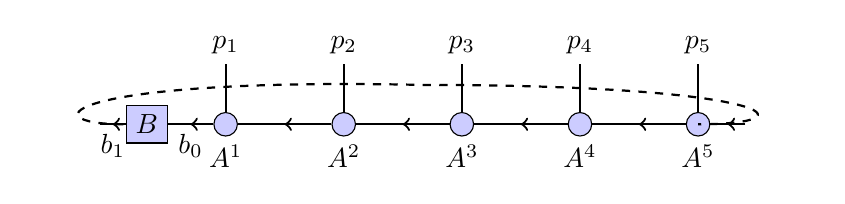
\begin{tikzpicture}[node distance=0.4cm]
\begin{scope}[decoration={
    markings,
    mark=at position 0.5 with {\arrow{>}}}
    ]
\foreach \i in {1,...,5} {
	\node[gamma] (G\i) at (1.5*\i,0) {};
	\node (l\i) at ($ (G\i) + (0, 1) $) {$p_\i$};
	\draw[thick] (G\i) -- (l\i);
	\node[below of=G\i] {$A^\i$};
}
\foreach \i / \j in {1/2,2/3,3/4,4/5} {
	\draw[thick, postaction={decorate}] (G\j) -- (G\i);
}
\node[side] (B) at (0.5, 0) {$B$};
%\node (b1) at (0, 0) {$b_1$};
\draw[thick, postaction={decorate}] (G1) -- node[below]{$b_0$}(B);
\draw[thick, postaction={decorate}] (8.1, 0)--(G5.east);
\draw[thick, postaction={decorate}] (B.west) -- node[below]{$b_1$}(-0.1, 0);
\end{scope}
\draw[thick, dashed] (0.2,0) .. controls (-1,0) and (-0.6,0.6) .. (4,0.5) .. controls (8.5,0.5) and (9,0) .. (7.5,0);
\end{tikzpicture}
    }
\end{figure}

\only<2>{
$$
\ket{\psi} = \sum\limits_{p_1 ... p_5}   Tr(B A^{p_1}_1 ... A^{p_5}_5)\ket{p_1 ... p_5} 
$$
}

}
\only<3->{
Every state has a matrix product state representation formed through the process of repeated SVD.

\only<3>{
\begin{figure}[h]
    \centering
    \scalebox{1.1}{
    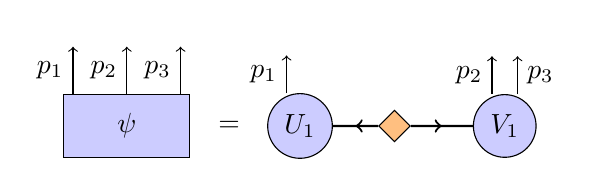
\begin{tikzpicture}[node distance=0.6cm]

\node[side, minimum width=1.6cm, minimum height=0.8cm] (psi) at (0,0) {$\psi$};
\node[above=of psi.north west, anchor=south west] (p1) {};
\node[above=of psi](p2) {};
\node[above=of psi.north east, anchor=south east] (p3) {};
\node at (1.3, 0) {=}; 
\node[cside] (psi1) at (2.2,0) {$U_1$};
\node[lambda] (S) at (3.4, 0) {};
\node[cside] (psiR) at (4.8,0) {$V_1$};
\node[above=of psi1.north west, anchor=south west] (pL) {};
\node[above=of psiR.north west, anchor=south west] (q2) {};
\node[above=of psiR.north east, anchor=south east] (qR) {};

\begin{scope}[decoration={
    markings,
    mark=at position 0.5 with {\arrow{>}}}
    ]
 \draw[->] (psi.north -| p1) -- node[left] {$p_1$} (p1);
 \draw[->] (psi) --  node[left] {$p_2$} (p2);
 \draw[->] (psi.north -| p3) -- node[left] {$p_3$} (p3);
 \draw[->] (psi1.north -| pL) -- node[left] {$p_1$} (pL);
 \draw[->] (psiR.north-|q2)-- node[left] {$p_2$} (q2);
 \draw[->] (psiR.north -| qR) -- node[right] {$p_3$} (qR);
 \draw[-, thick, postaction={decorate}]  (S) -- (psi1);
 \draw[-, thick, postaction={decorate}] (S) -- (psiR);
 \end{scope}
 \end{tikzpicture}
    }
    \note{Maximum bond dimension d}
\end{figure}
}
\only<4>{
\begin{figure}[h]
    \centering
    \scalebox{1.1}{
    \input{diagrams/mps3_2.tex}
    }
    \note{Maximum bond dimension d^2}
\end{figure}
}
\only<5>{
\begin{figure}[h]
    \centering
    \scalebox{1.1}{
    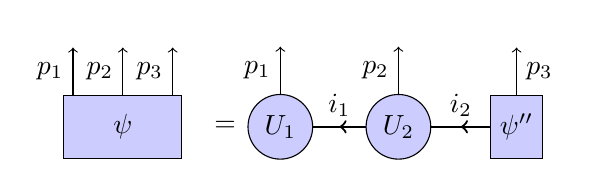
\begin{tikzpicture}[node distance=0.6cm]
    \node[side, minimum width=1.5cm, minimum height=0.8cm] (psi) at (0,0) {$\psi$};
    \node[above=of psi.north west, anchor=south west] (p1) {};
    \node[above=of psi](p2) {};
    \node[above=of psi.north east, anchor=south east] (p3) {};
    \node at (1.3, 0) {=};
    \node[cside] (B1) at (2,0) {$U_1$};
    \node[cside] (B2) at (3.5,0) {$U_2$};
    \node[side, minimum width=0.5cm, minimum height=0.8cm](psiR) at (5, 0){$\psi''$};
    %\node[lambda] (S) at (3, 0) {};
    %\node[side,minimum width=1cm, minimum height=0.8cm] (psiR) at (4.2,0) {$\psi'$};
    \node[above=of B1.north, anchor=south] (pL) {};
    \node[above=of B2] (q2) {};
    %\node[above=of psiR.north west, anchor=south west] (q2) {};
    \node[above=of psiR.north, anchor=south] (qR) {};
\begin{scope}[decoration={
    markings,
    mark=at position 0.5 with {\arrow{>}}}
    ]
    \draw[->] (psi.north -| p1) -- node[left] {$p_1$} (p1);
    \draw[->] (psi) --  node[left] {$p_2$} (p2);
    \draw[->] (psi.north -| p3) -- node[left] {$p_3$} (p3);
    \draw[->] (B1.north -| pL) -- node[left] {$p_1$} (pL);
    \draw[->] (B2.north-|q2)-- node[left] {$p_2$} (q2);
    \draw[->] (psiR.north -| qR) -- node[right] {$p_3$} (qR);
    \draw[-, thick, postaction={decorate}] (B2) -- node[above]{$i_1$}(B1);
    \draw[-, thick, postaction={decorate}] (psiR) -- node[above]{$i_2$}(B2);
 %\draw[-] (psiR) -- (S);
  \end{scope}
\end{tikzpicture}
    }
\end{figure}
}
}

\end{frame}
\begin{frame}{Tensor Network States}
\vskip-1.5cm
\begin{columns}[T]
\begin{column}[T]{.5\textwidth}
\bi
\item MPS and the generalization to PEPS automatically satisfy area law.

\item Entanglement rank and entropy bounded by total bond dimension across any cut.

\item Can view PEPS on cylinder as a MPS.
\ei 
\end{column}
\begin{column}{.5\textwidth}
\vskip-0.7cm
\begin{figure}
\includegraphics[width=6cm]{diagrams/CylPEPS1.png}
\caption{Translationally symmetric PEPS on a cylinder}
\end{figure}
\vskip-0.6cm
\begin{figure}
\includegraphics[width=2cm]{diagrams/CylPEPS2.png}
\caption{Close-up of site-tensor in PEPS}
\end{figure}
\end{column}
\end{columns}
\end{frame}
\begin{frame}{Computing Correlation Functions in MPS}
\vskip-1.5cm
\only<1,3->{
\begin{figure}[t]
\centering
\includegraphics[width=\textwidth]{diagrams/orus-corrfunc.pdf}
%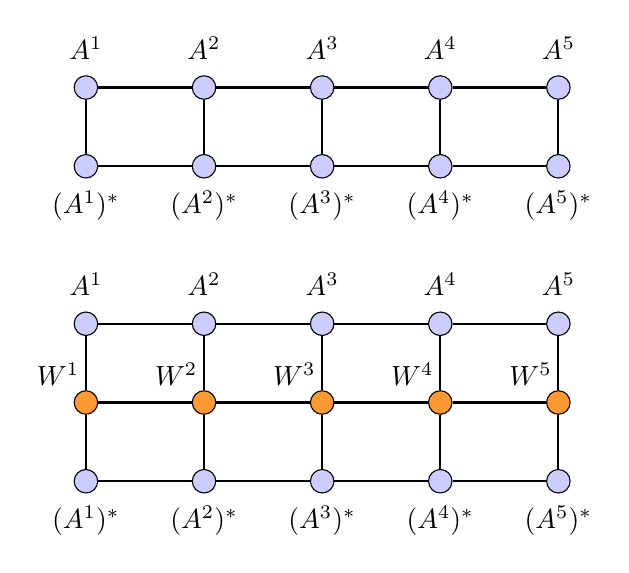
\begin{tikzpicture}[node distance=0.5cm]

\foreach \i in {1,...,5} {
	\node (Gp\i) at (1.5*\i,-2.5) [gamma] {};
	\node (Gpp\i) at ($ (Gp\i) + (0,-1) $) [gamma] {};
	\draw[thick] (Gp\i) -- (Gpp\i);
	\node[above of=Gp\i] {$A^\i$};
	\node[below of=Gpp\i] {$(A^\i)^*$};
}
\foreach \i / \j in {1/2,2/3,3/4,4/5} {
	\draw[thick] (Gp\i) -- (Gp\j);
	\draw[thick] (Gpp\i) -- (Gpp\j);
}

\foreach \i in {1,...,5} {
	\node (Gp\i) at (1.5*\i,-5.5) [gamma] {};
	\node (Gpp\i) at ($ (Gp\i) + (0,-2) $) [gamma] {};
	\node (O\i) at ($ (Gp\i) + (-0,-1) $) [operator] {};
	
	\draw[thick] (Gp\i) -- (O\i);
	\draw[thick] (Gpp\i) -- (O\i);
	
	\node[above of=Gp\i] {$A^\i$};
	\node[below of=Gpp\i] {$(A^\i)^*$};
	\node[above left of=O\i] {$W^\i$};
}
\foreach \i / \j in {1/2,2/3,3/4,4/5} {
	\draw[thick] (Gp\i) -- (Gp\j);
	\draw[thick] (Gpp\i) -- (Gpp\j);
	\draw[thick] (O\i) -- (O\j);
}

\end{tikzpicture}

\caption{Diagram for $C_{O O'}(r) = \ev{O_i O'_{i+r}}- \ev{O_i}\ev{O'_{i+r}}$}
\end{figure}
}
\only<2>{
\begin{columns}[T]
    \begin{column}[T]{.28\textwidth}
        \begin{figure}[h]
            \centering
            \scalebox{1}{
            \input{diagrams/transfer_matrix.tex}
            }
            \caption{Transfer Matrix $\mathbb{E}_{I}$}
            \note{Reminder using arrows to represent in and out}
        \end{figure}
    \end{column}
    \begin{column}[T]{.3\textwidth}
        \begin{figure}[h]
            \centering
            \scalebox{1}{
            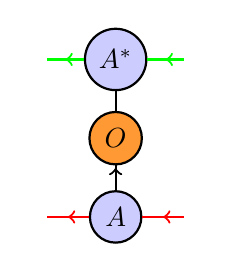
\begin{tikzpicture}[node distance=0.4cm]
\begin{scope}[thick, decoration={
    markings,
    mark=at position 0.5 with {\arrow{>}}}
    ]
  \node[gamma] (A) at (0,0) {$A$};  
  \node[operator] (O) at (0, 1) {$O$};
 % \node[operator] (O2) at (0, 1) {$O'$};
  \node[gamma] (Ac) at (0,2) {$A^{*}$};
  \draw[postaction={decorate}] (A)-- (O) -- (Ac);
  \node[inv] (ki) at (1, 0){};
  \node[inv] (bi) at (1, 2){}; 
  \node[inv] (ko) at (-1, 0){}; 
  \node[inv] (bo) at (-1, 2){};
  \draw[color=red, postaction={decorate}] (ki)--(A);
  \draw[color=green, postaction={decorate}] (bi)--(Ac);
  \draw[color=red, postaction={decorate}] (A) -- (ko);
  \draw[color=green, postaction={decorate}] (Ac) -- (bo);

\end{scope}
\end{tikzpicture}
            }
            \caption{Operator Insertion $\mathbb{E}_{O}$}
        \end{figure}
    \end{column}
    \begin{column}[T]{.42\textwidth}
        \vskip1.8cm
        \begin{figure}[h]
            \centering
            \scalebox{0.8}{
            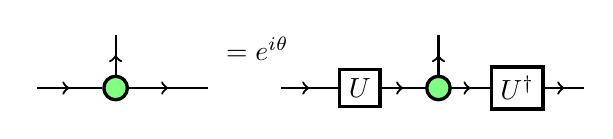
\begin{tikzpicture}
\begin{scope}[very thick,decoration={
    markings,
    mark=at position 0.5 with {\arrow{>}}}
    ] 

\node[peps] (A1) at (-4.1, 0) {};
\node (li) at ($(A1) + (-1, 0) $) {};
\draw[thick, postaction={decorate}] (li.center) -- (A1.west);
\draw[thick, postaction={decorate}] (A1.east) -- node[right] {} +(1,0);
\draw[thick, postaction={decorate}] (A1.north) -- node[above] {} +(0,0.5);

\node at (-2.3, 0.5){$= e^{i \theta}$};    

\node[peps] (A) at (0, 0) {};
\node[draw] (Ul) at ($(A) + (-1, 0) $) {$U$};
\node[draw] (Ur) at ($(A) + (1, 0) $) {$U^{\dagger}$};
\node (LI) at ($(Ul) + (-1, 0) $) {};
\draw[thick, postaction={decorate}] (LI.center) -- (Ul.west);
\draw[thick, postaction={decorate}] (Ur.east) -- node[right] {} +(0.5,0);
\draw[thick, postaction={decorate}] (Ul) -- (A);
\draw[thick, postaction={decorate}] (A) -- (Ur);
\draw[thick, postaction={decorate}] (A.north) -- node[above] {} +(0,0.5);

\end{scope}
\end{tikzpicture}
            }
            \caption{MPS gauge redundancy}
        \end{figure}
    \end{column}
\end{columns} 
\begin{figure}[h]
    \centering
    \scalebox{1}{
    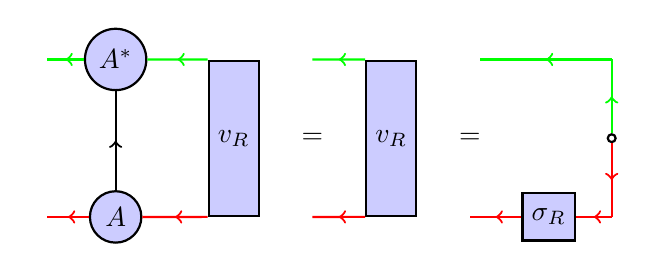
\begin{tikzpicture}[node distance=0.4cm]
\begin{scope}[thick, decoration={
    markings,
    mark=at position 0.5 with {\arrow{>}}}
    ]
  \node[gamma] (A) at (0,0) {$A$};  
  \node[gamma] (Ac) at (0,2) {$A^{*}$};
  \node[side, minimum height=1.97cm] (vR) at (1.5, 1){$v_R$};
  \draw[postaction={decorate}] (A)--(Ac);
  \node[inv] (ki) at (1, 0){};
  \node[inv] (bi) at (1, 2){}; 
  \node[inv] (ko) at (-1, 0){}; 
  \node[inv] (bo) at (-1, 2){};
  \draw[color=red, postaction={decorate}] (vR.south west) -- (ki.center)--(A);
  \draw[color=green, postaction={decorate}] (vR.north west)-- (bi.center)--(Ac);
  \draw[color=red, postaction={decorate}] (A) -- (ko);
  \draw[color=green, postaction={decorate}] (Ac) -- (bo);
  
  \node[] at (2.5, 1){$=$};
  \node[side, minimum height=1.97cm] (vR) at (3.5, 1){$v_R$};
  \node[inv] (ki) at (2.5, 0){};
  \node[inv] (bi) at (2.5, 2){};
  \draw[color=red, postaction={decorate}] (vR.south west) -- (ki.center);
  \draw[color=green, postaction={decorate}] (vR.north west)-- (bi.center); 

  \node[] at (4.5, 1){$=$};
  \node[side, minimum height=0.6cm] (sR) at (5.5, 0){$\sigma_R$};
  \node[inv] (ki) at (4.5, 0){};
  \node[inv] (k2) at (6.3, 0){};
  \node[cdot] (dot) at (6.3, 1){};
   \node[inv] (b2) at (6.3, 2){};
  \node[inv] (bi) at (4.5, 2){};
  \draw[color=red, postaction={decorate}]  (dot)--(k2.center);
  \draw[color=red, postaction={decorate}]  (k2.center)-- (sR.east);
  \draw[color=red, postaction={decorate}]  (sR.west) -- (ki.center);
  \draw[color=green, postaction={decorate}]  (dot)--(b2.center);
  \draw[color=green, postaction={decorate}]  (b2.center)-- (bi);
\end{scope}
\end{tikzpicture}
    }
\caption{Eigenvector equation $\mathbb{E}_{I}(\sigma_R) = \sigma_R$}
\end{figure}
   
}
\only<3>{
\vskip-0.5cm
 $$\ev{O_i O'_{i+r}} = \vbraopket{v_L}{\mathbb{E}_O \mathbb{E}_I^r \mathbb{E}_{O'}}{v_R}$$
 $$
 \lim\limits_{r \rightarrow \infty} \ev{O_i O'_{i+r}} = \vbraopket{v_L}{\mathbb{E}_O}{v_R} \vbraopket{v_L}{\mathbb{E}_{O'}}{v_R}
 $$
 $$ C_{O O'}(r) \approx const. \times \lambda_2^r $$
\note{Matrix product states also known as finitely correlated states}
}
\end{frame}

\begin{frame}{Computing Entanglement in MPS}
\vskip-1.5cm
To compute the spectrum of the reduced density matrix 
\begin{figure}
\scalebox{1}{
            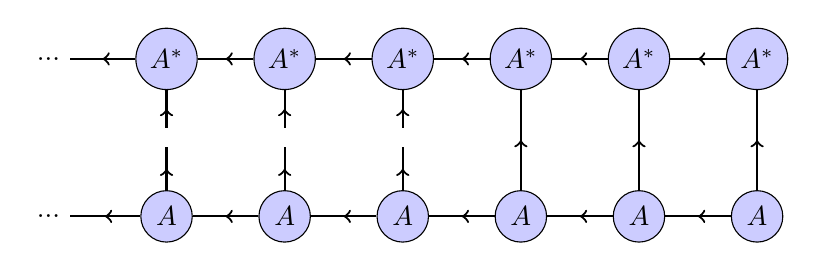
\begin{tikzpicture}[node distance=0.4cm]
\begin{scope}[decoration={
    markings,
    mark=at position 0.5 with {\arrow{>}}}
    ]
\foreach \i in {1,...,3} {
	\node[gamma] (G\i) at (1.5*\i,0) {$A$};
	\node (l\i) at ($ (G\i) + (0, 1) $) {$$};
	\draw[thick, postaction={decorate}] (G\i) -- (l\i);
	%\node[below of=G\i] {$A$};
}
\foreach \i / \j in {1/2,2/3} {
	\draw[thick, postaction={decorate}] (G\j) -- (G\i);
}
\node (b0) at (0, 0) {$...$};
\draw[thick, postaction={decorate}] (G1) -- (b0);

\foreach \i in {1,...,3} {
	\node[gamma] (B\i) at (1.5*\i,2) {$A^*$};
	\node (l\i) at ($ (B\i) + (0, -1) $) {$$};
	\draw[thick, postaction={decorate}] (l\i) -- (B\i);
	%\node[below of=G\i] {$A$};
}
\foreach \i / \j in {1/2,2/3} {
	\draw[thick, postaction={decorate}] (B\j) -- (B\i);
}
\node (b1) at (0, 2) {$...$};
\draw[thick, postaction={decorate}] (B1) -- (b1);

\foreach \i in {4,...,6} {
	\node[gamma] (G\i) at (1.5*\i,0) {$A$};
	\node[gamma] (B\i) at (1.5*\i,2) {$A^*$};
	\draw[thick, postaction={decorate}] (G\i) -- (B\i);
	}
\foreach \i / \j in {3/4,4/5,5/6} {
	\draw[thick, postaction={decorate}] (G\j) -- (G\i);
	\draw[thick, postaction={decorate}] (B\j) -- (B\i);
}
\end{scope}
\end{tikzpicture}

            }
\end{figure}

\only<1>{
Step 1. Show that the following matrix $\mathcal{U}$ is isometric.
\begin{figure}
\scalebox{1}{
            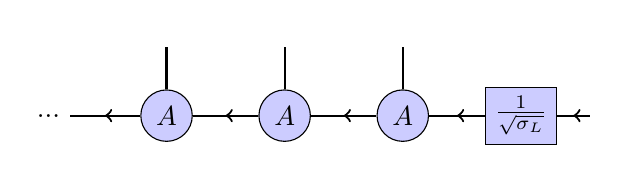
\begin{tikzpicture}[node distance=0.4cm]
\begin{scope}[decoration={
    markings,
    mark=at position 0.5 with {\arrow{>}}}
    ]
\foreach \i in {1,...,3} {
	\node[gamma] (G\i) at (1.5*\i,0) {$A$};
	\node (l\i) at ($ (G\i) + (0, 1) $) {$$};
	\draw[thick] (G\i) -- (l\i);
	%\node[below of=G\i] {$A$};
}
\foreach \i / \j in {1/2,2/3} {
	\draw[thick, postaction={decorate}] (G\j) -- (G\i);
}
\node (b0) at (0, 0) {$...$};
\node[side, minimum height=0.7cm] (sigL) at (6, 0) {$\frac{1}{\sqrt{\sigma_L}}$};
\draw[thick, postaction={decorate}] (G1) -- (b0);
\draw[thick, postaction={decorate}] (sigL) -- (G3);
\node[inv](Q) at (7, 0){};
\draw[thick, postaction={decorate}] (Q) -- (sigL);
\end{scope}
\end{tikzpicture}

            }
\end{figure}
}

\only<2>{
Step 2. Insert identity... 

}
\only<3->{

Result: 
$$\rho_L = \mathcal{U} \sqrt{\sigma_L} \sigma_R \sqrt{\sigma_L} \mathcal{U^{\dagger}}$$ 

To get the spectrum, we only need to compute the much smaller matrix 
$$\tilde{\rho}_L =  \sqrt{\sigma_L} \sigma_R \sqrt{\sigma_L} $$

}
\end{frame}
\begin{frame}{PEPS Construction of Honeycomb F.B.I.}
\vskip-1.5cm
A wavefunction written as a product of local operators acting on a product state can be turned into a tensor network.

\only<1>{
\begin{figure}[h]
\scalebox{1}{
% y=\sqrt{3/4}*(minimum size)/2
%

%http://tex.stackexchange.com/questions/6019/drawing-hexagons
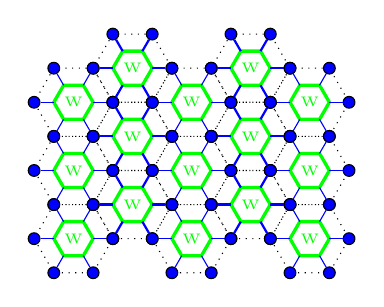
\begin{tikzpicture}[x=7.5mm,y=4.33mm]
  % some styles
  \tikzset{
    box/.style={
      regular polygon,
      regular polygon sides=6,
      minimum size=10mm,
      inner sep=0mm,
      outer sep=0mm,
      rotate=0,
     dotted,
     thin,
      black,
      draw
    }
  }
  \tikzset{
    bbox/.style={
      regular polygon,
      regular polygon sides=6,
      minimum size=7mm,
      %fill,
      inner sep=0mm,
      outer sep=0mm,
      rotate=0,
     % dotted,
     very thick,
     orange,
      draw
    }
  }
    \tikzset{
    wb/.style={
       regular polygon,
      regular polygon sides=6,
      minimum size=5mm,
      %fill,
      inner sep=0mm,
      outer sep=0mm,
      rotate=0,
     % dotted,
     very thick,
     green,
      draw
    }
  }
 \tikzset{boson/.style={circle=1pt,draw=black!100,fill=orange!100,inner sep=2pt}}
  \tikzset{dimer/.style={ellipse=1pt,draw=black!100,fill=orange!90,inner sep=2pt}}
    \tikzset{thindimer/.style={ellipse=1pt,draw=black!100,fill=orange!90,inner sep=1pt}}
\tikzset{peps/.style={circle=2pt,draw=black!100,fill=green!50,inner sep=3pt}}
\tikzset{bpeps/.style={circle=2pt,draw=black!100,thick,fill=green!50,inner sep=3pt}}
\tikzset{gamma/.style={circle=2pt,draw=black!100,fill=blue!50,inner sep=3pt}}
\tikzset{lambda/.style={rectangle,rotate=45,draw=black!100,fill=red!50,inner sep=2pt}}
\tikzset{operator/.style={circle=1pt,draw=black!100,fill=blue,inner sep=1.5pt}}

\foreach \i in {0,...,2} 
    \foreach \j in {0,...,2} {
    \pgfmathtruncatemacro{\x}{2*\i}
    \pgfmathtruncatemacro{\y}{2*\j}
            \node[box] (H\x\y) at (\x,\y) {};
             \node[wb] (W\x\y) at (\x,\y) {};
              \node[green] at (\x, \y) {\tiny W};
             \foreach \k in {1, ..., 6}{
             \node[operator] (D\x\y\k) at (H\x\y.corner \k) {};
             \draw[ blue] (W\x\y) -- (D\x\y\k);
             }
        }
\foreach \i in {0,1} 
    \foreach \j in {0,..., 2} {
        \pgfmathtruncatemacro{\x}{2*\i+1}
    \pgfmathtruncatemacro{\y}{2*\j+1}
   	  \node[box] (H\x\y) at (\x,\y) {};   
   	   \node[wb] (W\x\y) at (\x,\y) {};
   	    \node[green] at (\x, \y) {\tiny W};
             \foreach \k in {1, ..., 6}{
             \node[operator] (D\x\y\k) at (H\x\y.corner \k) {};
             \draw[thick, blue] (W\x\y) -- (D\x\y\k);
             }
        }


            %\foreach \k in {1,...,6}{
          %  \node[circle, label=above:\i, fill=red] at (H\i\j.corner \k) {};
           % }
%\node[circle, draw] at (H00.corner 1) {};
\end{tikzpicture}
}
\end{figure}

Virtual W-state on each plaquette used to synchronize the creation operators in the sum $\sum\limits_{i \in \varhexagon} b^{\dagger}_i$
$$\vket{W} = \vket{000001}+\vket{000010}+\vket{000100}+\vket{001000}+\vket{010000}+\vket{100000}$$

}

\only<2>{
\begin{columns}[T]
\begin{column}{0.5\textwidth}
\begin{figure}[h]
\scalebox{1.3}{
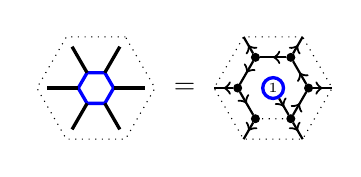
\begin{tikzpicture}[x=7.5mm,y=4.33mm]
\begin{scope}[decoration={
    markings,
    mark=at position 0.5 with {\arrow{>}}}
    ]
    
  \tikzset{
    box/.style={
      regular polygon,
      regular polygon sides=6,
      minimum size=15mm,
      inner sep=0mm,
      outer sep=0mm,
      rotate=0,
     dotted,
     thin,
      black,
      draw
    }
    }
      \tikzset{
    abox/.style={
      regular polygon,
      regular polygon sides=6,
      minimum size=9mm,
      inner sep=0mm,
      outer sep=0mm,
      rotate=0,
     dotted,
     thin,
      black,
      draw
    }
    }


    \tikzset{
    wb/.style={
       regular polygon,
      regular polygon sides=6,
      minimum size=4.5mm,
      %fill,
      inner sep=0mm,
      outer sep=0mm,
      rotate=0,
     % dotted,
     very thick,
     blue,
      draw
    }
  }
\tikzset{smalldot/.style={circle=1pt,draw=black!100,fill=black!100,inner sep=1pt}}
\tikzset{smallwdot/.style={circle=1pt, very thick, draw=blue!100,fill=white,inner sep=1pt}}

 \node[box] (H) at (0, 0) {};
\node[wb] (W) at (0,0) {};

\foreach \k in {1, ..., 6}{
             \node[inv] (D\k) at (H.corner \k) {};
             \draw[very thick, black] (W) -- (D\k);
             }
             
 \node[] at (1.5, 0){$=$};

 \node[box] (H3) at (3, 0) {};
 \node[abox] (H2) at (3, 0) {};
%\node[wb] (W) at (3,0) {\tiny W};
\foreach \k in {1, ..., 6}{
             \node[smalldot] (A\k) at (H2.corner \k) {};
             }

\foreach \k in {1,2,3,5}{
		\pgfmathtruncatemacro{\j}{\k+1}
            \draw[thick, postaction={decorate}] (A\k) -- (A\j);
             }
             \draw[thick, postaction={decorate}] (A6) -- (A1);
             
 \foreach \k in {1,2,3,4,5,6}{
            \draw[thick, postaction={decorate}] (A\k) -- (H3.corner \k);
             }
             
 \node[smallwdot](B) at (3, 0) {\tiny 1};
 \draw[thick, postaction={decorate}]  (B)--(A5);

\end{scope}
\end{tikzpicture}
}
\end{figure}
$$\vket{W} = \vket{100...}+...$$
\vskip-0.5cm
\bi 
\item W-State can be factored and put on hexagon sites
\item Each black directed string has either charge $0$ or $1$
\item Charge conserved
\ei 
\end{column}
\begin{column}{0.5\textwidth}
\begin{figure}[h]
\scalebox{1.5}{
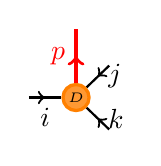
\begin{tikzpicture}[x=7.5mm,y=4.33mm]
\begin{scope}[decoration={
    markings,
    mark=at position 0.5 with {\arrow{>}}}
    ]
    

\tikzset{operator/.style={circle=1pt,draw=orange!100, very thick, fill=orange!80,inner sep=1pt}}
   
   \node[operator] (A) at (1, 0){\tiny $D$};
    \draw[thick, postaction={decorate}] (0.2, 0) --node[below]{$i$} (A);
    \draw[thick, postaction={decorate}] (5/3.2, 3/3.2) -- node[right]{$j$}(A);
    \draw[thick, postaction={decorate}] (5/3.2, -3/3.2) -- node[right]{$k$} (A);
    \draw[red, very thick, postaction={decorate}]  (A)-- node[left]{$p$}(1, 2);




\end{scope}
\end{tikzpicture}
}
\end{figure}
\vskip-0.3cm
\bi 
\item `Projects' the three virtual qubits coming into each vertex on to a state in physical Hilbert space
\item Physical state is either $\ket{0}, \ket{1}, \ket{2}, \ket{3}$
\item Charge conserved
\ei 
\end{column}
\end{columns}
}

\end{frame}
\begin{frame}{Correlations in Honeycomb F.B.Is}
\vskip-1.5cm
\only<1>{
\begin{figure}[hbctp]
\begin{center}
\includegraphics[width=8cm]{{summary/log_bdagb_corr_comparison.pdf}}
\end{center}
\caption{The correlation function $<b_x b^{\dagger}_0>$ shown on a log-scale F.B.I. and hard-core projected version.}
\end{figure}
}
\only<2>{

\begin{figure}[hbctp]
\begin{center}
\includegraphics[width=5cm]{diagrams/corrlengthbound.png}
\end{center}
\end{figure}

Evidence for energy gap - exponentially decaying correlations in thermodynamic limit
}
\end{frame}
\section{Entanglement Edge of Honeycomb Insulators}

\begin{frame}{Zig-zag Edge Entanglement Cut}
\vskip-1.5cm
\begin{figure}[h]
\scalebox{1}{
\input{diagrams/FI_PEPS_cut.tex}
}
\end{figure}
\bi 
\item Cylinder, Circumference $L$
\item Cut crosses $L$ W-strings
\item $\widetilde{\rho} = \exp{-\widetilde{H}}$ is a density matrix on $L$ spin 1/2s 
\ei 
\end{frame}

%\subsection{CFT Identification}
\begin{frame}{Entanglement Spectra}
\vskip-1.5cm
\only<1>{
\begin{figure}
\includegraphics[width=\textwidth]{{interpolatedboson/new_plots/L_10_all_mom_10.pdf}}
\end{figure}
}
\only<2>{
\begin{figure}[hbctp]
\begin{center}
\includegraphics[width=\textwidth]{{interpolatedboson/new_plots/L_9_all_mom_10.pdf}}
\end{center}
\end{figure}}
\end{frame}
\begin{frame}{Finite Size Analysis of Spectra}
\vskip-1.5cm
\begin{columns}[T]
    \begin{column}{.4\textwidth}
        \bi 
        \item<1-> Topological entanglement entropy is 0 
        \item<2-> Low energy modes show gapless $1/L$ behavior
        \ei
    \end{column}
    \begin{column}{.6\textwidth}
    \vskip-.3cm
        \only<2>{
        \begin{figure}[hbctp]
        \centering
        \includegraphics[width=2.5in]{{interpolatedboson/a10/plots/EntanglementEnergyScaling2.pdf}}
        %\caption{Power law fits for the lowest three states above the ground state at momentum zero and lowest two states at momentum 1 in Figure \ref{fig:sc-EEFinitesize}. The $1/L$ scaling is a signature of a gapless (entanglement) Hamiltonian. The labeling of the states $\ket{e, m}$ or $j_{-1} \ket{e, m}$ is explained in the CFT section below.}
        %\label{fig:sc-EEScaling}
        \end{figure}
        }
    \end{column}
\end{columns}
\end{frame}
\include{slides/CFT_EE}
\begin{frame}{Level identification in CFT spectra}
\vskip-1.5cm
\only<1>{

To make a precise comparison with the free-boson CFT, we'll need to solve for (or look up) the solution of this model.

The free-boson CFT is created from the Lagrangian 
$$ \mathfrak{L} = \frac{g}{2}\int dt \int\limits_0^L dx ( \frac{1}{v^2}(\partial_t \phi)^2 - (\partial_x \phi)^2)$$
and with the compatified field identification
$$ \phi \equiv \phi + 2\pi R$$
and placed on the circle of circumference $L$ with periodic boundary conditions
$$ \phi(x) \equiv \phi(x+L).$$
}

Canonically quantize!
\end{frame}
\begin{frame}{Conformal Tower}
\only<1>{
\begin{figure}
    \scalebox{1}{
        \input{diagrams/CFT_tower1.tex}
    }
\end{figure}
}
\only<2>{
\begin{figure}
    \scalebox{1}{
        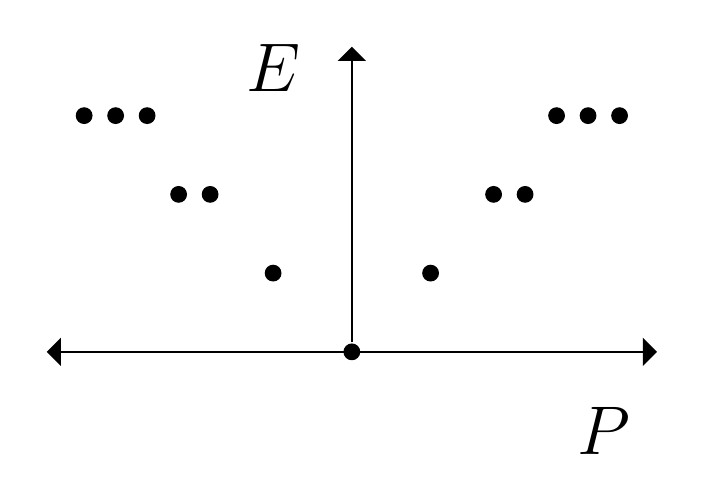
\begin{tikzpicture}
\tikzstyle{yaxis} = [-triangle 90]
\tikzstyle{xaxis} = [triangle 90-triangle 90]
\node[inv](A) at (-4, 0){};
\node[inv](B) at (4, 0){};
\draw[thick, xaxis] (A)-- (B);
\node at ($ (A) !.9! (B) +(0, -1)$) {\Huge $P$};
\node[inv](A) at (0, 0){};
\node[inv](B) at (0, 4){};
\draw[thick, yaxis] (A)--(B);
\node at ($ (A) !.9! (B) +(-1, 0)$) {\Huge $E$};

\tikzset{spec/.style={circle=2pt,draw=black!100,fill=black!100,inner sep=2pt}}
\node[spec] at (0, 0){};
\node[spec] at (1, 1){};
\node[spec] at (1.8, 2){};
\node[spec] at (2.2, 2){};

\node[spec] at (2.6, 3){};
\node[spec] at (3.0, 3){};
\node[spec] at (3.4, 3){};

\node[spec] at (-1, 1){};
\node[spec] at (-1.8, 2){};
\node[spec] at (-2.2, 2){};

\node[spec] at (-2.6, 3){};
\node[spec] at (-3.0, 3){};
\node[spec] at (-3.4, 3){};


%\node[spec] at (-1, 1){};
%\node[spec] at (0, 2){};

%\node[] at (3, -1.5){\LARGE Band metal};
%\node[] at (3, 1.5){\LARGE Band insulator};
%\draw[] (0.5, 0) -- (5.5, 0);
\end{tikzpicture}
    }
\end{figure}
}
\only<3>{
\begin{figure}
    \scalebox{1}{
        \input{diagrams/CFT_tower3.tex}
    }
\end{figure}
}
\only<4>{
\begin{figure}
    \scalebox{1}{
        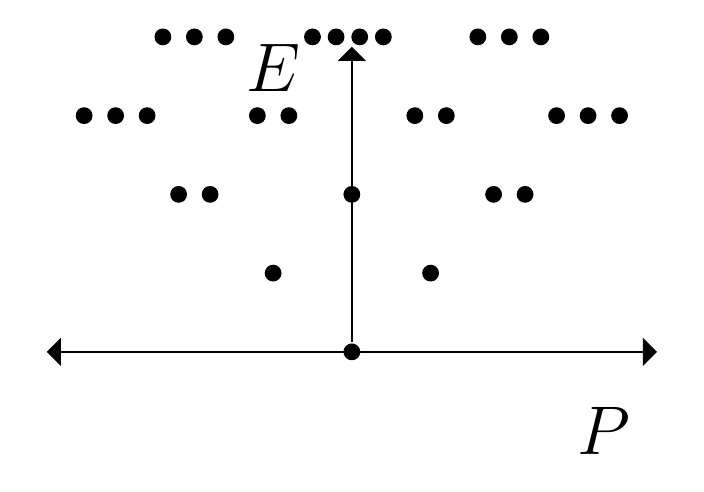
\begin{tikzpicture}
\tikzstyle{yaxis} = [-triangle 90]
\tikzstyle{xaxis} = [triangle 90-triangle 90]
\node[inv](A) at (-4, 0){};
\node[inv](B) at (4, 0){};
\draw[thick, xaxis] (A)-- (B);
\node at ($ (A) !.9! (B) +(0, -1)$) {\Huge $P$};
\node[inv](A) at (0, 0){};
\node[inv](B) at (0, 4){};
\draw[thick, yaxis] (A)--(B);
\node at ($ (A) !.9! (B) +(-1, 0)$) {\Huge $E$};

\tikzset{spec/.style={circle=2pt,draw=black!100,fill=black!100,inner sep=2pt}}
\node[spec] at (0, 0){};
\node[spec] at (1, 1){};
\node[spec] at (1.8, 2){};
\node[spec] at (2.2, 2){};

\node[spec] at (2.6, 3){};
\node[spec] at (3.0, 3){};
\node[spec] at (3.4, 3){};

\node[spec] at (0-1, 0+1){};
\node[spec] at (1-1, 1+1){};
\node[spec] at (1.8-1, 2+1){};
\node[spec] at (2.2-1, 2+1){};

\node[spec] at (2.6-1, 3+1){};
\node[spec] at (3.0-1, 3+1){};
\node[spec] at (3.4-1, 3+1){};

\node[spec] at (0-2.2, 0+2){};
\node[spec] at (1-2.2, 1+2){};
\node[spec] at (1.8-2.3, 2+2){};
\node[spec] at (2.2-2.1, 2+2){};

\node[spec] at (0-1.8, 0+2){};
\node[spec] at (1-1.8, 1+2){};
\node[spec] at (1.8-2, 2+2){};
\node[spec] at (2.2-1.8, 2+2){};

\node[spec] at (-2.6, 3){};
\node[spec] at (-3.0, 3){};
\node[spec] at (-3.4, 3){};

\node[spec] at (-2.6+1, 4){};
\node[spec] at (-3.0+1, 4){};
\node[spec] at (-3.4+1, 4){};


\end{tikzpicture}
    }
\end{figure}
}
\end{frame}
\newcommand{\uL}{\mathbf{L_0}}
\newcommand{\bL}{\mathbf{\bar{L}_0}}
\begin{frame}{Level identification in CFT spectra}
\vskip-1.5cm
\begin{table}[h]
\centering
\begin{tabular}{c|c}

$\mathbf{P} =\frac{2\pi}{L}(\uL-\bL)$ & 
$\frac{2\pi}{L}(em + n - \bar{n})$ \\
&
\\
$\widetilde{\mathbf{P}}$  &
$(em + n - \bar{n})$\\
& 
\\
$\mathbf{H} = \frac{2\pi}{L}(\uL+\bL)$ &
 $\frac{2\pi}{L}(\frac{\kappa e^2}{2} + \frac{m^2}{2 \kappa} + \frac{n + \bar{n}}{2})$ \\
&
 \\
$\widetilde{\mathbf{H}} = \frac{L}{2 \pi \kappa}\mathbf{H}$ &
 $e^2 + \frac{m^2}{4 \kappa^2} + \frac{1}{\kappa}(n + \bar{n})$       
\end{tabular}
\label{Table:EV}
\caption{Eigenvalues of states $\ket{e, m}_{n, \bar{n}}$.} 
\end{table}

The rescaled Hamiltonian $\widetilde{\mathbf{H}}$ has eigenvalues that depend on only one free-parameter, $\kappa = 1/(4 \pi g R^2)$.

\end{frame}

\begin{frame}{Level identification in CFT spectra}
\vskip-1.5cm
\begin{figure}
\scalebox{0.5}{
\input{diagrams/CFT_schematic3.tex}
}
\end{figure}
\end{frame}
%%\newcommand{\uL}{\mathbf{L_0}}
%\newcommand{\bL}{\mathbf{\bar{L}_0}}
\begin{frame}{Level identification in CFT spectra}
\vskip-1.5cm

\end{frame}
\begin{frame}{Goals for Honeycomb Mott Insulator}
\vskip-1.5cm
\begin{block}{Completed}
\bi 
\item Build a tensor network representation for doing computations
\item  Verify that no spontaneous symmetry breaking occurs
%We'll do this by computing correlation functions on a cylinder geometry combined with scaling analysis in the circumference

\item Rule out topological order

\item Compute entanglement spectrum to check for nontrivial entanglement

\ei 
\end{block}
\begin{block}{Not Yet}
\bi
\item Understand the role of symmetries in protecting entanglement in interacting quasi-1D and 2D theories
\item Find distinguishing topological invariant and/or physical signatures
\item Find a parent Hamiltonian 
\ei
\end{block}
\end{frame}
\begin{frame}{Open questions and speculation}
\bi
\item Parent Hamiltonian - Construct or obstruction?
\item Symmetry group/groups that protect edge?
\item Correspondence between bulk perturbations and edge perturbations?
\item Nearby phase transitions? 
\item Is the edge `anomalous'? 
\item We can put lots of known SPTs in tensor networks. What should we do next?
\item Can we represent transfer matrix as a MPO for efficient contraction?
\item Tensor Network RG?
\ei 

\end{frame}
\section*{}

\begin{frame}
  \frametitle{Resources}
  %\framesubtitle{If you want to improve this style}
  \begin{thebibliography}{10}

  \beamertemplatearticlebibitems

  \bibitem{PEPS}
  A Practical Introduction to Tensor Networks
    \newblock {\tt Orus, R. A Practical Introduction to Tensor Networks: Matrix Product States and Projected Entangled Pair States. arXiv [cond-mat.str-el] (2013). at <http://arxiv.org/abs/1306.2164> 
}

  \end{thebibliography}
\end{frame}

\frame{
  \vspace{2cm}
  {\huge Questions ?}

  \vspace{3cm}
  \begin{flushright}
    Brayden Ware

    \structure{\footnotesize{brayden@physics.ucsb.edu}}
  \end{flushright}
}

\frame{
  \vfill
  \centering
  \highlighton{
  \usebeamerfont*{frametitle}Bonus slides

  \usebeamerfont*{framesubtitle}Bonus slides
  }
  \vfill
}

\begin{frame}{Bulk Entanglement and Edges}
%We can (heuristically for now) connect the existence of the edge state to the idea that these types of insulators are really distinct from atomic insulators. 
\vskip-1.5cm
Bulk ground state contains information about edge physics
\bi
\item  Imagine cutting IQH state in half, forming edge states $\ket{k}_{L, R}$
%or another state with a protected edge
%at this point, the eigenstates of the system are factored between left and right sides
% the lowest energy states look like ground states far away, but differ at the edge due to the edge modes 
\item Adiabatically tune the coupling back to normal value 
%and find the new ground state
\item System can lower its energy by coupling the currents
\item Entangled eigenstate $\sum \ket{k}_L \otimes\ket{-k}_R$ 
% But this is just the regular state of the system with no cut at all!
\item Atomic insulator wavefunctions factor trivially - no entanglement.
% This suggests that these are distinct phases of matter from atomic insulators, we should look at entanglement and show that the entanglement is robust to perturbations. This can be a route to showing the edge is robust to (certain) perturbations without having to worry about the actual precise form of the edge.  
\ei 
\vskip-0.2cm
\begin{figure}
\includegraphics[width=\linewidth]{diagrams/entanglement_cut.png}
\end{figure}
\footnotetext[3]{
\citep{Alexandradinata2011-os}} 
\end{frame}


\begin{frame}{MPS Example: AKLT State}
\vskip-1.5cm
\begin{block}{Haldane Phase for Spin-1 chains $(j=1, m=0)$}
\vskip-0.8cm
$$
H_{AKLT} = \sum\limits_{i} J \vec{S}_i\cdot \vec{S}_{i+1} + J' (\vec{S}_i\cdot \vec{S}_{i+1})^2 + D (S^z_i)^2+BS^x
$$
\end{block}
\begin{columns}[T]
    \begin{column}[T]{.45\textwidth}
        \vskip-1.2cm
        \begin{figure}
        \centering
        \includegraphics[width=\columnwidth]{diagrams/aklt2.png}
        \end{figure}
    \end{column}
    \begin{column}[T]{.55\textwidth}
    \vskip-0.8cm
    Two distinct featureless insulators:
    \bi 
    \item Large-D phase
    \bi 
    \item Contains product state wavefunction $\ket{\psi} = \ket{000...}$ 
    \ei
    \item Haldane phase
    \bi 
    \item Contains AKLT wavefunction $\ket{\psi} = \Sigma\ket{+00-0+...}$
    \ei 
        \begin{figure}[h]
            \hspace{-2cm}
            \scalebox{1.2}{
            \begin{frame}{MPS Example: AKLT State}
\vskip-1.5cm
\begin{block}{Haldane Phase for Spin-1 chains $(j=1, m=0)$}
\vskip-0.8cm
$$
H_{AKLT} = \sum\limits_{i} J \vec{S}_i\cdot \vec{S}_{i+1} + J' (\vec{S}_i\cdot \vec{S}_{i+1})^2 + D (S^z_i)^2+BS^x
$$
\end{block}
\begin{columns}[T]
    \begin{column}[T]{.45\textwidth}
        \vskip-1.2cm
        \begin{figure}
        \centering
        \includegraphics[width=\columnwidth]{diagrams/aklt2.png}
        \end{figure}
    \end{column}
    \begin{column}[T]{.55\textwidth}
    \vskip-0.8cm
    Two distinct featureless insulators:
    \bi 
    \item Large-D phase
    \bi 
    \item Contains product state wavefunction $\ket{\psi} = \ket{000...}$ 
    \ei
    \item Haldane phase
    \bi 
    \item Contains AKLT wavefunction $\ket{\psi} = \Sigma\ket{+00-0+...}$
    \ei 
        \begin{figure}[h]
            \hspace{-2cm}
            \scalebox{1.2}{
            \begin{frame}{MPS Example: AKLT State}
\vskip-1.5cm
\begin{block}{Haldane Phase for Spin-1 chains $(j=1, m=0)$}
\vskip-0.8cm
$$
H_{AKLT} = \sum\limits_{i} J \vec{S}_i\cdot \vec{S}_{i+1} + J' (\vec{S}_i\cdot \vec{S}_{i+1})^2 + D (S^z_i)^2+BS^x
$$
\end{block}
\begin{columns}[T]
    \begin{column}[T]{.45\textwidth}
        \vskip-1.2cm
        \begin{figure}
        \centering
        \includegraphics[width=\columnwidth]{diagrams/aklt2.png}
        \end{figure}
    \end{column}
    \begin{column}[T]{.55\textwidth}
    \vskip-0.8cm
    Two distinct featureless insulators:
    \bi 
    \item Large-D phase
    \bi 
    \item Contains product state wavefunction $\ket{\psi} = \ket{000...}$ 
    \ei
    \item Haldane phase
    \bi 
    \item Contains AKLT wavefunction $\ket{\psi} = \Sigma\ket{+00-0+...}$
    \ei 
        \begin{figure}[h]
            \hspace{-2cm}
            \scalebox{1.2}{
            \input{diagrams/aklt.tex}
            }
        \end{figure}

    \ei
    \end{column}
\end{columns}

\end{frame}
            }
        \end{figure}

    \ei
    \end{column}
\end{columns}

\end{frame}
            }
        \end{figure}

    \ei
    \end{column}
\end{columns}

\end{frame}
\begin{frame}{1D SPT Example: AKLT State}
\vskip-1.5cm
\only<1>{
\begin{figure}
\scalebox{2}{
            \begin{frame}{MPS Example: AKLT State}
\vskip-1.5cm
\begin{block}{Haldane Phase for Spin-1 chains $(j=1, m=0)$}
\vskip-0.8cm
$$
H_{AKLT} = \sum\limits_{i} J \vec{S}_i\cdot \vec{S}_{i+1} + J' (\vec{S}_i\cdot \vec{S}_{i+1})^2 + D (S^z_i)^2+BS^x
$$
\end{block}
\begin{columns}[T]
    \begin{column}[T]{.45\textwidth}
        \vskip-1.2cm
        \begin{figure}
        \centering
        \includegraphics[width=\columnwidth]{diagrams/aklt2.png}
        \end{figure}
    \end{column}
    \begin{column}[T]{.55\textwidth}
    \vskip-0.8cm
    Two distinct featureless insulators:
    \bi 
    \item Large-D phase
    \bi 
    \item Contains product state wavefunction $\ket{\psi} = \ket{000...}$ 
    \ei
    \item Haldane phase
    \bi 
    \item Contains AKLT wavefunction $\ket{\psi} = \Sigma\ket{+00-0+...}$
    \ei 
        \begin{figure}[h]
            \hspace{-2cm}
            \scalebox{1.2}{
            \begin{frame}{MPS Example: AKLT State}
\vskip-1.5cm
\begin{block}{Haldane Phase for Spin-1 chains $(j=1, m=0)$}
\vskip-0.8cm
$$
H_{AKLT} = \sum\limits_{i} J \vec{S}_i\cdot \vec{S}_{i+1} + J' (\vec{S}_i\cdot \vec{S}_{i+1})^2 + D (S^z_i)^2+BS^x
$$
\end{block}
\begin{columns}[T]
    \begin{column}[T]{.45\textwidth}
        \vskip-1.2cm
        \begin{figure}
        \centering
        \includegraphics[width=\columnwidth]{diagrams/aklt2.png}
        \end{figure}
    \end{column}
    \begin{column}[T]{.55\textwidth}
    \vskip-0.8cm
    Two distinct featureless insulators:
    \bi 
    \item Large-D phase
    \bi 
    \item Contains product state wavefunction $\ket{\psi} = \ket{000...}$ 
    \ei
    \item Haldane phase
    \bi 
    \item Contains AKLT wavefunction $\ket{\psi} = \Sigma\ket{+00-0+...}$
    \ei 
        \begin{figure}[h]
            \hspace{-2cm}
            \scalebox{1.2}{
            \input{diagrams/aklt.tex}
            }
        \end{figure}

    \ei
    \end{column}
\end{columns}

\end{frame}
            }
        \end{figure}

    \ei
    \end{column}
\end{columns}

\end{frame}
            }
\end{figure}
\begin{columns}[T]
\begin{column}[T]{.5\textwidth}
\vskip-1.5cm
\begin{figure}
\includegraphics[width=\columnwidth]{diagrams/aklt2.png}
\end{figure}
\end{column}
   \begin{column}[T]{.5\textwidth}
   \vskip-1cm
    \includegraphics[width=\columnwidth]{diagrams/akltEE.png}
    \end{column}
\end{columns}
}
Haldane phase distinguished by exact double degeneracy in entire  entanglement spectrum.

\only<2>{
\begin{figure}
\includegraphics[width=\textwidth]{diagrams/akltchart.png}
\end{figure}
}
\end{frame}
\begin{frame}{Technical Slide: Threading Flux in a MPS}


\end{frame}
\begin{frame}{Flux-Threading Arguments for SPTs?}
\vskip-1.5cm
Recall that the boundary conditions in a MPS are set by a matrix at the edge.

\begin{figure}[h]
    \centering
    \scalebox{1}{
    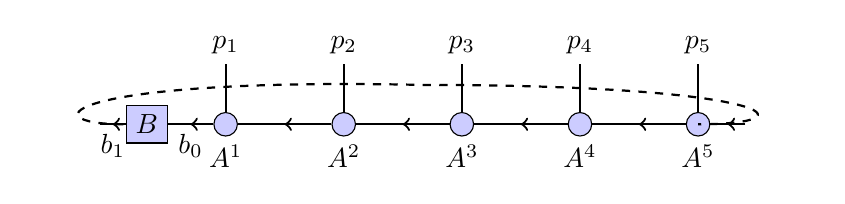
\begin{tikzpicture}[node distance=0.4cm]
\begin{scope}[decoration={
    markings,
    mark=at position 0.5 with {\arrow{>}}}
    ]
\foreach \i in {1,...,5} {
	\node[gamma] (G\i) at (1.5*\i,0) {};
	\node (l\i) at ($ (G\i) + (0, 1) $) {$p_\i$};
	\draw[thick] (G\i) -- (l\i);
	\node[below of=G\i] {$A^\i$};
}
\foreach \i / \j in {1/2,2/3,3/4,4/5} {
	\draw[thick, postaction={decorate}] (G\j) -- (G\i);
}
\node[side] (B) at (0.5, 0) {$B$};
%\node (b1) at (0, 0) {$b_1$};
\draw[thick, postaction={decorate}] (G1) -- node[below]{$b_0$}(B);
\draw[thick, postaction={decorate}] (8.1, 0)--(G5.east);
\draw[thick, postaction={decorate}] (B.west) -- node[below]{$b_1$}(-0.1, 0);
\end{scope}
\draw[thick, dashed] (0.2,0) .. controls (-1,0) and (-0.6,0.6) .. (4,0.5) .. controls (8.5,0.5) and (9,0) .. (7.5,0);
\end{tikzpicture}
    }
\end{figure}

Inserting the group operation $V_g$ on a single link in a periodic chain is the same as changing the boundary conditions. This is an operational procedure for 'threading a flux' that works in interacting theories or even with then symmetry is inversion or time-reversal.

The edge action can be interpreted as a 'composition of fluxes' $V_g V_h = \exp{i \omega(g, h)} V_{gh}$.
\end{frame}
\begin{frame}{Symmetry Protected Entanglement}
\vskip-1.5cm
\bi 
\item These edge symmetries $V_g$ commute with the 'reduced density matrix' $\tilde{\rho}_L$ of the system and thus only act non-trivially on degenerate entanglement spectra eigenvalues. 

\item Because the classes of projective symmetry groups are discrete, you can't change the action on the edge continuously between classes (without going through a phase transition.)
\ei 
\begin{figure}
\includegraphics[width=\textwidth]{diagrams/akltchart.png}
\end{figure}
\end{frame}
\begin{frame}{Properties of Featureless MPS}
\vskip-1.5cm

\begin{alert}{Make this more brief, move details to end}
Boil down to we can determine the symmetry properties
Show pictures of what it looks like for symmetry to act on the edge of the chain, say what it means for schmidt states
\end{alert}

MPS for featureless 1D or quasi-1D systems have non-degenerate transfer matrices and are called simple. Simple MPS can be proved to have:

\bi 
\item Correlations are insensitive to boundary conditions
\item Can construct a featureless 'parent Hamiltonian' 
\note{from the wavefunction alone}
\item Two simple MPS with equal wavefunctions are (uniquely) gauge equivalent
\item Corollary: Edges can be labeled with a (possibly projective) representation of the group of physical symmetries.

\begin{figure}
\scalebox{1}{
            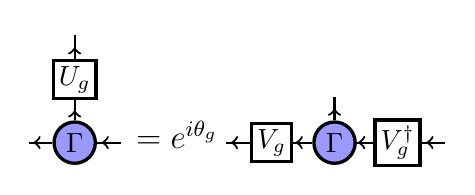
\begin{tikzpicture}
\tikzset{gamma/.style={circle=2pt,draw=black!100, very thick, fill=blue!40, inner sep=2pt}}
\tikzset{box/.style={draw, inner sep = 2pt}}
\begin{scope}[very thick,decoration={
    markings,
    mark=at position 0.5 with {\arrow{<}}}
    ] 
    
\pgfmathsetmacro{\left}{-1.3}
\pgfmathsetmacro{\center}{0}
\pgfmathsetmacro{\right}{2}

\pgfmathsetmacro{\bond}{0.3}

\node[box] (Ug) at (\left, 0.8) {$U_g$};
\node[gamma] (A1) at (\left, 0) {$\Gamma$};

\draw[thick, postaction={decorate}] ($(A1.west) + (-\bond, 0) $) -- (A1.west);
\draw[thick, postaction={decorate}] (A1.east) -- node[right] {} +(\bond,0);


\node at (\center, 0.1){\large $ = e^{i \theta_g}$};    


\node[gamma] (A) at (\right, 0) {$\Gamma$};
\node[box] (VL) at ($(A) + (-0.8, 0) $) {$V_{g}$};
\node[box] (VR) at ($(A) + (0.8, 0) $) {$V_{g}^{\dagger}$};
\draw[thick, postaction={decorate}]  ($(VL.west)+(-\bond, 0)$) -- (VL.west);
\draw[thick, postaction={decorate}] (VR.east) -- ($(VR.east)+(\bond, 0)$);
\draw[thick, postaction={decorate}] (VL) -- (A);
\draw[thick, postaction={decorate}] (A) -- (VR);

\end{scope}
\begin{scope}[very thick,decoration={
    markings,
    mark=at position 0.5 with {\arrow{>}}}
    ] 
\pgfmathsetmacro{\bond}{0.3}
\draw[thick, postaction={decorate}] (A1)--(Ug);
\draw[thick, postaction={decorate}] (Ug.north) -- node[above] {} +(0,\bond);
\draw[thick, postaction={decorate}] (A.north) -- node[above] {} +(0,\bond);
\end{scope}
\end{tikzpicture}
            }
\end{figure}

\item Bonus: we can determine $V_g$ by diagonalizing the transfer matrix with the insertion $U_g$. 

\ei 

\note{
Transfer matrix becomes degenerate when 
\bi 
\item 
\item Correlations in spontaneous symmetry breaking MPS have extreme senstivity to boundary conditions
\item Correlations in topological ordered state (on large enough cylinder) completely insensitive to boundary conditions when operators don't wrap around cylinder.
\item Gapless 2D PEPS on cylinder?

\item Notes on phase transitions in MPS?
\ei 
}
\end{frame}
\end{document}
